%\renewcommand{\chaptername}{Section}

%-----------------------------------------------------------------------------------------------------------------
%% Section 1 : Introduction
\chapter{Introduction}
	\label{chapt:intro}

Living in the era where it is nearly impossible to live without it, cellular service is very important. Up nearly 13\% from last year, it is said that US consumers are checking their mobile devices at a remarkable rate of 9 billion times per day \cite{deloittestat}.\\

It is numbers like these that have inspired \Company to begin research and development of the worlds first commercial, autonomous, aerostat's. Led by state of the art controls, Altaeros' mission is to help provide these services, including power in even the most remote of areas. The latest product is seen below in Figure~\ref{fig:1_companypic}~\cite{companypicweb}.

\begin{figure}[H]
	\centering
	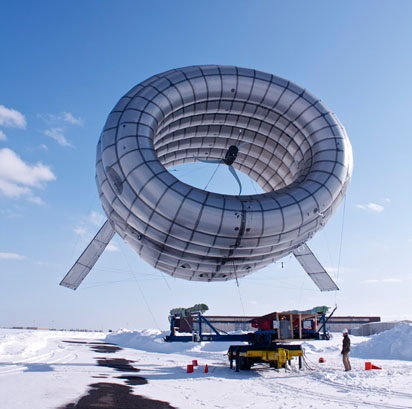
\includegraphics[width=0.6\textwidth]{1_companypic}
	\caption{Overview of Altaeros' aerostat.}\protect\cite{companypicweb}
	\label{fig:1_companypic}
\end{figure}


The above figure raises the question, how does this system remain stable. This is achieved through the system's tether management system.

\section{Background} % (fold)

The winch system is responible for the control of the aerostat. An overview of similar system used by Altaeros is shown below in Figure~\ref{fig:1_winch}~\cite{winchpic}.
\begin{figure}[H]
	\centering
	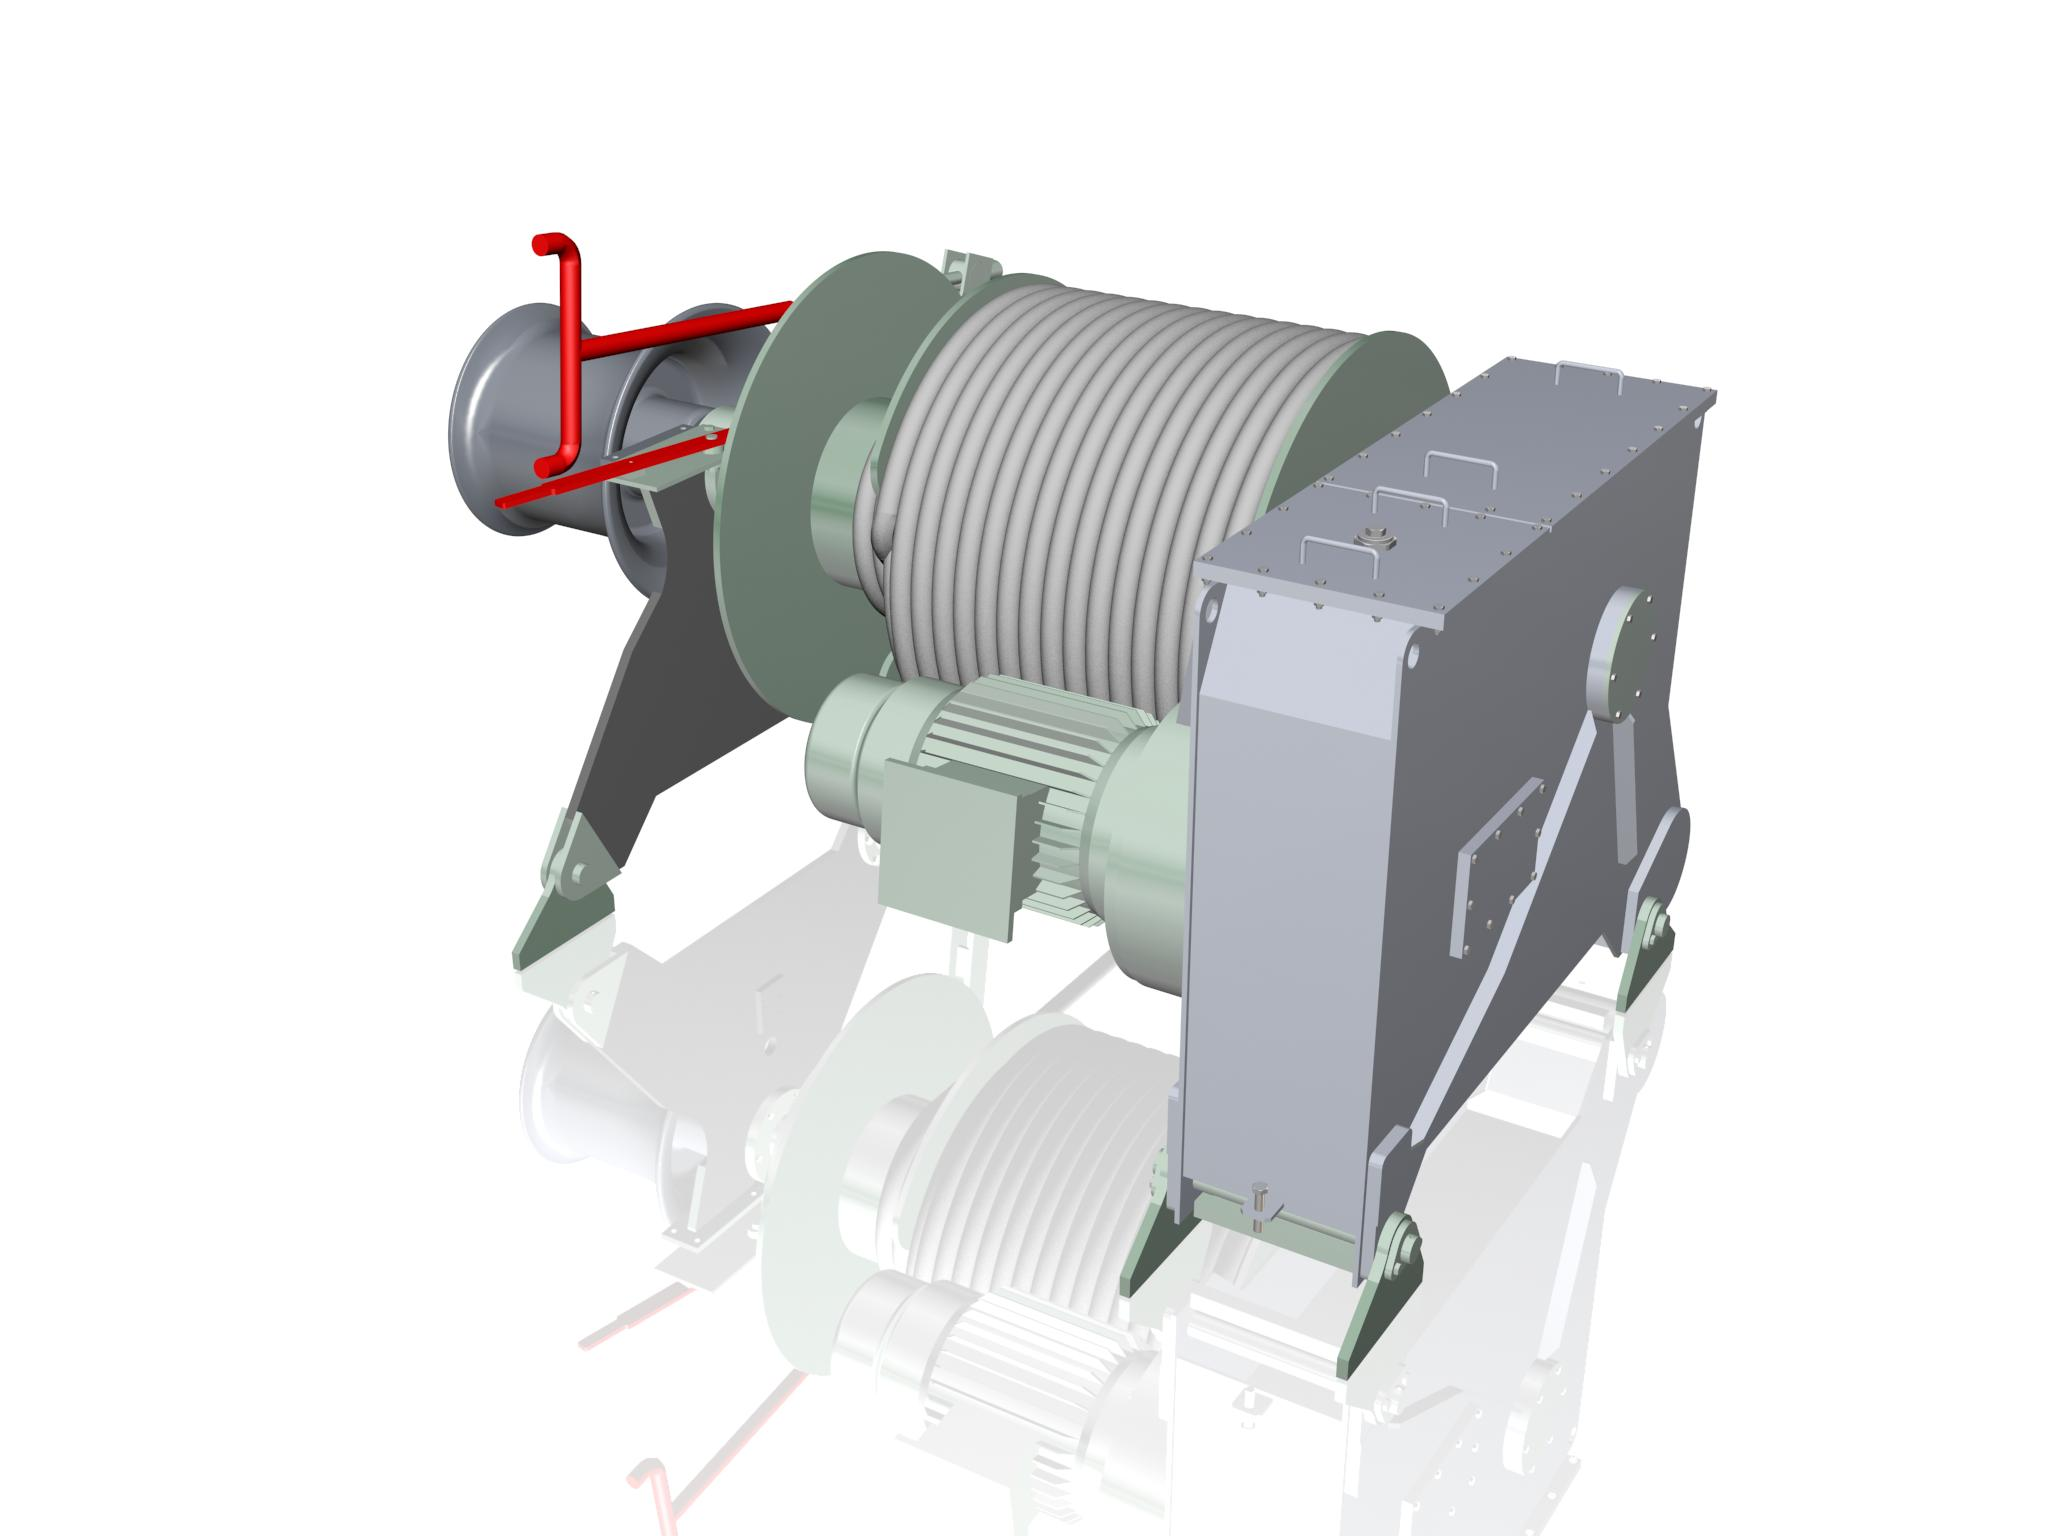
\includegraphics[scale=0.2]{1_winch}
	%% must use protect to put reference in caption
	\caption{Example of common winch system.}\protect\cite{winchpic}
	\label{fig:1_winch}
\end{figure}

It has been deemed that Altaeros could manufacture a more custom, cheaper and efficient winch system. In order to assure that the system is capable of handling the large aerodynamic loads translated by the tether, a complete structural analysis must be completed.

\section{Purpose}
The purpose of this report is to perform the structural analysis in order to assure that the winch drum assembly is capable of handling the large loads.\\

An overview of the winches drum assembly is shown from the 3D computer aided design (CAD) model developed with Inventor \cite{INVENTOR} as per Figure~\ref{fig:1_drum}.
\begin{figure}[H]
	\centering
	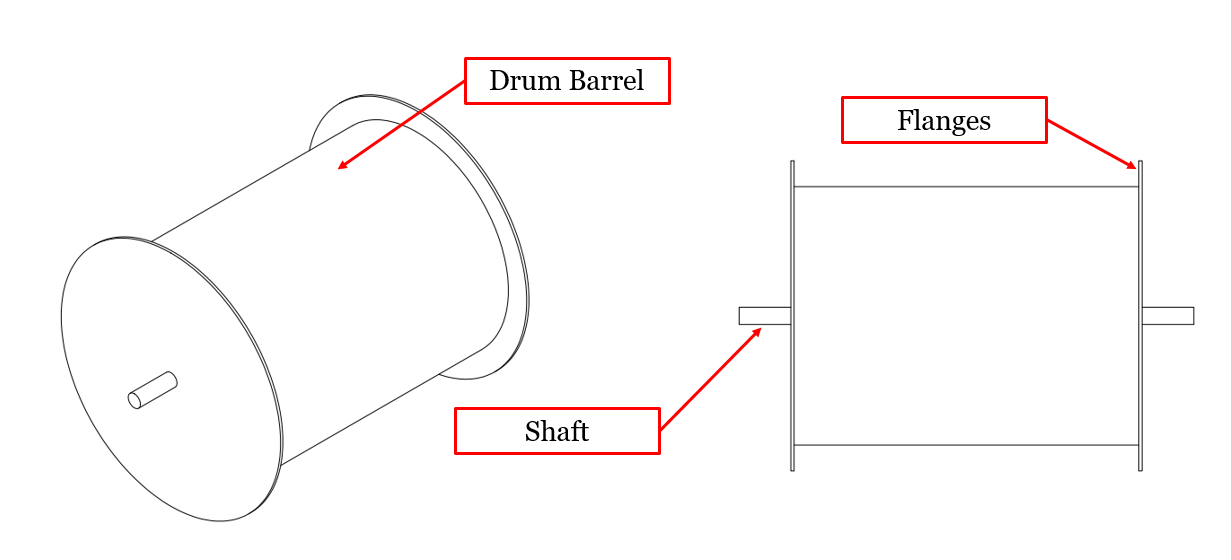
\includegraphics[scale=0.5]{1_drum}
	\caption{Drum assembly CAD model.}
	\label{fig:1_drum}
\end{figure}

It is important to realize that most of loading from the tether will be translated as pressure onto the barrel. This loading scenario will be investigated to properly size the winch barrel thicknesses which is the driving design dimension.

\section{Scope}

In the following sections of this report, the relevant parameters will be presented. From this, existing codes and standards will be investigated in exploring what a quick analysis would yield. From this, a more advanced numerical approach will be presented. These results will then be validated by use of finite element analysis (FEA). Finally, all results will be discussed, relevant conclusions and recommendations will be made.

%-----------------------------------------------------------------------------------------------------------------
%% Section 2 : Discussion
\chapter{Codes \& Standards}
	\label{chapt:standards}

Before any complex analysis is completed, initial existing codes and standards will be investigated.\\

The most important parameter in question is the outer diameter $D_o$. For this entire report, it will be assumed that this value is constant at $D_o = 711\ mm = 28\ in$. Based on this fixed parameter, the following relevant values which will be used in this report are summarized below in Table~\ref{table:prelim_params}. All material properties selected as per John Umina's  suggestion from Table 1A of \cite{ASMEbvpcIID} for a SA-106 Grade B steel (most commonly used in seamless pipe). Units shown in both metric (SI) and United States customary (USC).\\

\begin{table}[ht]
	\caption{Key drum parameters and material properties.}
	\centering
	%	\begin{tabular}{c c c c}
	%		%heading
	%		\hline \textbf{Description} & \textbf{Symbol} & \textbf{Value} & \textbf{Units}\\[1 ex]
	%		\hline
	%		%Main table body content	
	%		Outer diameter		&$D_o$			& $28$		& $in$ 	\\
	%		Tether diameter		&$D_{thr}$		& $0.6$		& $in$ 	\\
	%		Drum length			&$L$			& $49$		& $in$ 	\\
	%		Tether tension		&$T$			& $11,525$	& $lbf$	\\	
	%		Yield strength		&$S_y$			& $35,000$	& $psi$	\\	
	%		Young's Modulus		&$E$			& $2.9\cdot 10^7$ &$psi$\\
	%		Poisson's ratio		&$\nu$			& $0.3$		& $ul$	\\	
	%		\hline
	%	\end{tabular}
	\begin{tabular}{lccccc}
		&       & \multicolumn{2}{c}{\textbf{\textit{SI}}} & \multicolumn{2}{c}{\textbf{\textit{UCS}}} \\
		\textbf{Description} & \textbf{Symbol} & \textbf{Value} & \textbf{Units} & \textbf{Value}  & \textbf{Units} \\
		\midrule
		Outer diameter       & $D_o$           & $711.2$        & $mm$           & $28$            & $in$           \\
		Tether diameter      & $D_{thr}$       & $15.2$         & $mm$           & $0.598$         & $in$           \\
		Drum length          & $L$             & $1,244.6$      & $mm$           & $49$            & $in$           \\
		Tether tension       & $T$             & $51,264$       & $N$            & $11,525$        & $lbf$          \\
		Yield strength       & $S_y$           & $241.3$        & $MPa$          & $35,000$        & $psi$          \\
		Young's modulus      & $E$             & $200$          & $GPa$          & $2.9\cdot 10^7$ & $psi$          \\
		Poisson's ratio      & $\nu$           & $0.3$          & $-$            & $-$             & $-$            \\
		Safety factor        & $SF$            & $1.5$          & $-$            & $-$             & $-$            \\
	\end{tabular}%
	\label{table:prelim_params}
\end{table}

The best approach to this problem is to model the drum as an externally pressured vessel. First, in order to make this approximation, it is required to investigate how the tether tension is translated into an external pressure. This will be done by reviewing the derivation for the Capstan Equation.\\ 

Next, using the above mentioned parameters and pressure, it was suggested by John Umina that the following standards should be investigated.
\begin{itemize}
	\item American Society of Mechanical Engineers (ASME):
	      \begin{itemize}[label=$\bullet$]
	      	\item Boiler and Pressure Vessel Code, Section VIII, Division 1, 2015 \cite{ASMEbvpcVII1}
	      	\item Boiler and Pressure Vessel Code, Section VIII, Division 2, 2015 \cite{ASMEbvpcVII2}
	      \end{itemize}
	\item European Standard EN
	      \begin{itemize}[label=$\bullet$]
	      	\item EN 13445: Unfired Pressure Vessels, Part 3: Design,  2002 \cite{EN134453}
	      \end{itemize}
	\item Det Norske Veritas(DNV) \cite{DNVOSD101}
	      \begin{itemize}[label=$\bullet$]
	      	\item DNV-OS-D101, Marine and Machinery Systems and Equipment\cite{ASMEbvpcVII1}
	      \end{itemize}
	\item Thin Walled Pressure Vessel (TWPV) Hoop Stress \cite{roarks}\\	
\end{itemize}

It is to be noted that the same symbols used in the aforementioned references will be used in the foregoing sections for clarity.
%----------------------------------------------------------------------------------------------------------------------
\section{Capstan Equation}
It is required to understand how one wrap of tether in tension results in an external pressure $p$ applied to the outer surface of the cylinder.\\

After much research into this problem, the solution reveals itself into the derivation of the well-known Capstan Equation~\ref{eq:Capstan} \cite{capstanman}.

\begin{equation}
	\label{eq:Capstan}
	T_2 = T_1 e^{\mu\theta}
\end{equation}

Where $T_1$ is the hold force and $T_2$ is the pull force (i.e. $T_2 \geq T_1$). \\

From this equation, the free body diagram that leads to this solution is presented below in Figure~\ref{fig:Capstan}~\cite{capstanman}. 

\begin{figure}[H]
	\centering
	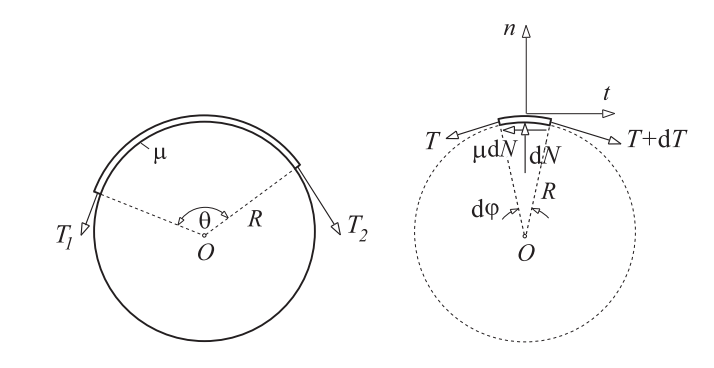
\includegraphics[scale=0.75]{2_Capstan}
	\caption{Free body diagram of differential capstan problem.}
	\label{fig:Capstan}
\end{figure}

Based on this, what is of question is how to extrapolate a pressure $p$ from the applied tension $T$. This can be done performing a force balance ($\Sigma F_{\hat{n}} = 0 $)in the normal direction $\hat{n}$ which reduces to Equation~\ref{eq:CapstanSigRad}.

\begin{equation}
	\label{eq:CapstanSigRad}
	dN-(T+dT)\sin \frac{d\varphi}{2}+T\sin \frac{d\varphi}{2}= 0
\end{equation}

By assuming a small change in angle, the substitution of $\sin \varphi \approx \varphi$ and $dT d\varphi/2 \approx 0$ are be made. Applying these relations to \ref{eq:CapstanSigRad} leaves \ref{eq:diffNormal}.

\begin{equation}
	\label{eq:diffNormal}
	dN = T d\varphi
\end{equation}

%%-----------------------------

Similarly, a force balance ($\Sigma F_{\hat{t}} = 0 $)in the tangential direction $\hat{t}$ which reduces to Equation~\ref{eq:CapstanSigTan}.

\begin{equation}
	\label{eq:CapstanSigTan}
	(T+dT)\cos \frac{d\varphi}{2}- T\cos \frac{d\varphi}{2} - \mu dN= 0
\end{equation}

Again, assuming a small change in angle ($\cos \varphi \approx 1$) to \ref{eq:CapstanSigTan} leads to \ref{eq:diffTens}.

\begin{equation}
	\label{eq:diffTens}
	dT = \mu dN
\end{equation}

From the above equation, it is now clear that the overall normal force $N$ caused by the tension $T$ can be solved for by integration \ref{eq:capstan_integral} yielding \ref{eq:CapstanNorm}.

\begin{equation}
	\label{eq:capstan_integral}
	\int_0^N dN =\int_0^{2\pi} T d\varphi
\end{equation}

\begin{equation}
	\label{eq:CapstanNorm}
	N=2\pi T	
\end{equation}

With this resultant normal force over one revolution of tether, it is now apparent that the pressure $p$ can be solved for by distributing $N$ over this area as seen in Equation~\ref{eq:2_preq}.

\begin{equation}
	\label{eq:2_preq}
	p=\frac{N}{A}=\frac{2\pi T}{d\pi D}=\frac{2T}{Dd}
\end{equation}

Using the values from Table~\ref{table:prelim_params} and \ref{eq:2_preq}, $p=1376\  psi= 9.484\  MPa$. 

%------------------------------------------------------------------------------------------
\subsection{Alternate Solution}
\label{subsection:alt}
By letting $T = T(\theta)= T_{hi} e^{-\mu \varphi}$, Equation~\ref{eq:capstan_integral} becomes \ref{eq:capstan_integral2} hence yielding \ref{eq:CapstanNorm2} (recall $\int e^{ax} dx = \frac{1}{a} e^{ax} + C$).

\begin{equation}
	\label{eq:capstan_integral2}
	\begin{aligned}
		\int_0^N dN =\int_0^{\theta} T_{hi} e^{-\mu \varphi} d\varphi            \\
		N = \left( -\frac{T_{hi}}{\mu} e^{-\mu \varphi} \right) \Big|_0^{\theta} 
	\end{aligned}
\end{equation}

\begin{equation}
	\label{eq:CapstanNorm2}
	N = \frac{T_{hi}}{\mu} \left( 1 - e^{-\mu \theta} \right)
\end{equation}

With this stored normal force, it is now the pressure $p$ after $\theta$ of contact angle,  can be solved for by distributing $N$ over this area (dependent on angle) as seen in Equation~\ref{eq:2_preq2}.

\begin{equation}
	\label{eq:2_preq2}
	p=\frac{N}{A}= \frac{T_{hi} \left( 1 - e^{-\mu \theta} \right)}{\mu d_{thr} R \theta}
\end{equation}

Using a script from Appendix~\ref{appendix:a0}, the following plots in Figures~\ref{fig:2_nvar} and \ref{fig:2_pvar} show the variation in normal force $N$ and pressure $p$ for different values of coefficient of friction $\mu$.

\begin{figure}[H]
	\centering
	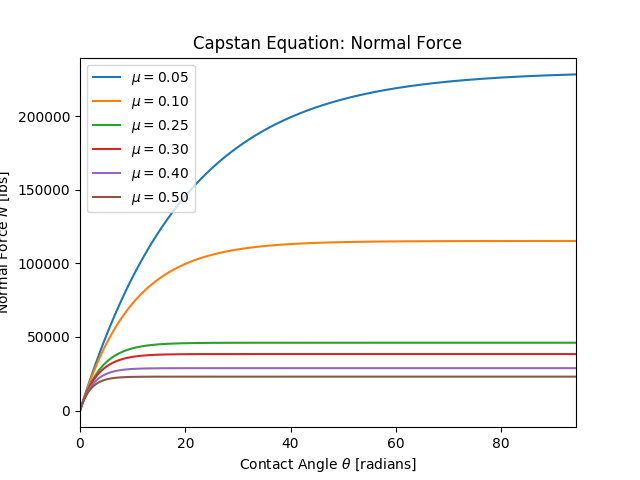
\includegraphics[scale=0.75]{2_nvar}
	\caption{Variation of stored normal force $N$ versus contact angle $\theta$.}
	\label{fig:2_nvar}
\end{figure}

\begin{figure}[H]
	\centering
	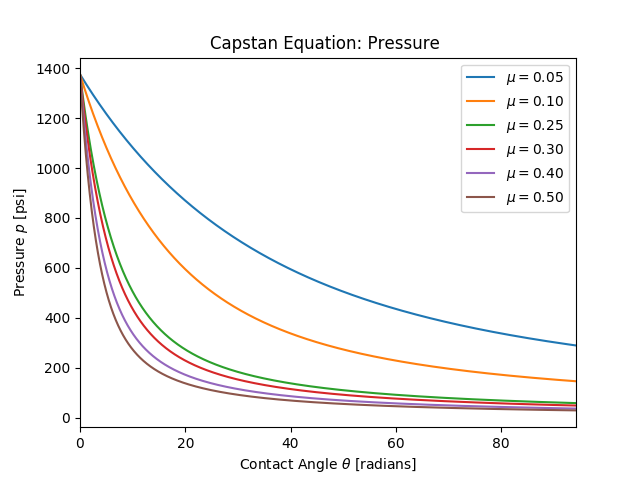
\includegraphics[scale=0.75]{2_pvar}
	\caption{Variation of pressure $p$ versus contact angle $\theta$.}
	\label{fig:2_pvar}
\end{figure}

It is clear from these plots that as the contact angle increases, the stored normal force has an asymptomatic behavior. This behavior coupled with the increase increase in area results in a pressure which goes to zero. Furthermore, as the coefficient of friction between the tether and the drum increases, the decay in pressure is quicker. A key observation to be made is that regardless of the $\mu$, all initial pressures $p(\theta)$ start at the value calculated from Equation~\ref{eq:2_preq}.  

%%----------------------------------------------------------------------------------------------------------------------
\section{ASME's BPVC}

The ASME codes listed in the beginning of this chapter will be extensively studied. Note that for all iteration procedures in this report, an initial thickness of $t_0 = 12.7\ mm=0.500\ in$ with a step of $t_0 = 0.254\ mm=0.01\ in$. Python scripts utilized for implementing solving algorithms can be found in Appendix~A developed with \cite{PYTHON}. 
\subsection{Section VIII: Division 1}
As per UG-28 of \cite{ASMEbvpcVII1}, the following procedure was used to calculate the required thickness.
The following list of steps were carried out as per \cite{ASMEbvpcVII1}.

\begin{enumerate}
	\item Assume initial thickness value of $t$
	\item Calculate $D_o/t$ ratio and assure $D_o/t \geq 10$.
	\item Calculate $L/D_o$ ratio, if $L/D_o \geq 50 \Rightarrow 50$ or  $L/D_o \leq 0.05 \Rightarrow 0.05$
	\item With above ratios, go to Figure G of \cite{ASMEbvpcIID} and get value for $A$
	\item With $A$ from above go to chart CS-2 $\because S_y \geq 30 \ ksi$ to get $B$
	\item Use Equation \ref{eq:2_VII1_pa} with $B$ to calculate allowable pressure $p_a$:
	      \begin{equation}
	      	\label{eq:2_VII1_pa}
	      	p_a = \frac{4B}{3 \left(D_o/t\right)}
	      \end{equation}
	\item Check that $p_a \geq p_{req}$ as calculated from Equation~\ref{eq:2_preq}, if not, increase $t$ and go to Step 2\\
	      	
\end{enumerate}

With the Python Script from Appendix~\ref{appendix:a1} the convergence plot from Figure~\ref{fig:2_vii1_cnvg} below was created.
\begin{figure}[H]
	\centering
	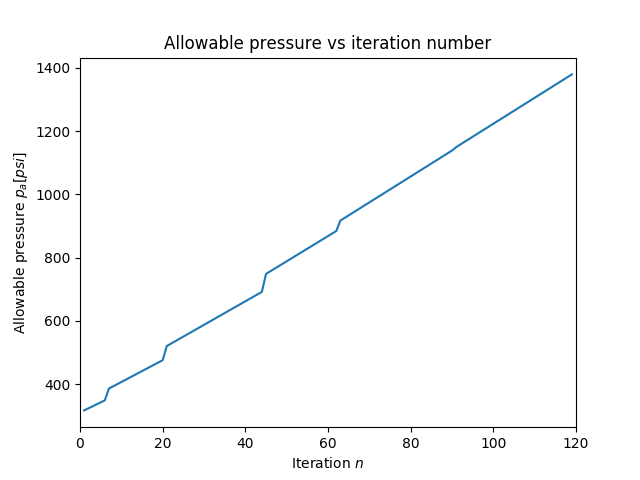
\includegraphics[scale=0.8]{2_vii1_cnvg}
	\caption{Convergence plot of $p_a$ using ASME's BPVC VIII-1.}
	\label{fig:2_vii1_cnvg}
\end{figure}

From this plot, the script converged at thickness of $t = 43.7\ mm = 1.68\ in$ and an allowable pressure of $p_a\geq p_{reqs}$ after $n=119$ iterations. 


\subsection{Section VIII: Division 2}
As per subsection 4.4.5 of \cite{ASMEbvpcVII2}, the following procedure was used to calculate the required thickness. Note that only the main formulas will be presented. For intermediate steps, see  the Python script in Appendix~\ref{appendix:a2}. The following list of steps were carried out as per \cite{ASMEbvpcVII2}.

\begin{enumerate}
	\item Assume initial thickness value of $t$
	\item Calculate elastic buckling stress $F_{he}$ with Equation~\ref{eq:2_VII2_4419}
	      \begin{equation}
	      	\label{eq:2_VII2_4419}
	      	F_{he} = \frac{1.6\ C_h E_y t}{D_o}
	      \end{equation}
	\item Based on $S_y$ and $F_{he}$, calculate the predicted buckling stress $F_{ic}$ \ref{eq:2_VII2_4419}
	\item With subsection 4.4.2 of \cite{ASMEbvpcVII2}, compute the design factor $FS$
	\item Calculate allowable pressure $p_a$ with Equation~\ref{eq:2_VII2_4428}
	      \begin{equation}
	      	\label{eq:2_VII2_4428}
	      	p_a = 2 F_{ha} \left(\frac{t}{D_o}\right)
	      \end{equation}
	\item Check if $p_a \geq p_{req}$ as calculated from \ref{eq:2_preq}, if not, increase $t$ and go to Step 2 \\
	      	
\end{enumerate}

%%on page~\pageref{fig:2_vii2_cnvg} for page ref
The Python Script in Appendix~\ref{appendix:a2} output the following convergence plot as seen in Figure~\ref{fig:2_vii2_cnvg}.
\begin{figure}[H]
	\centering
	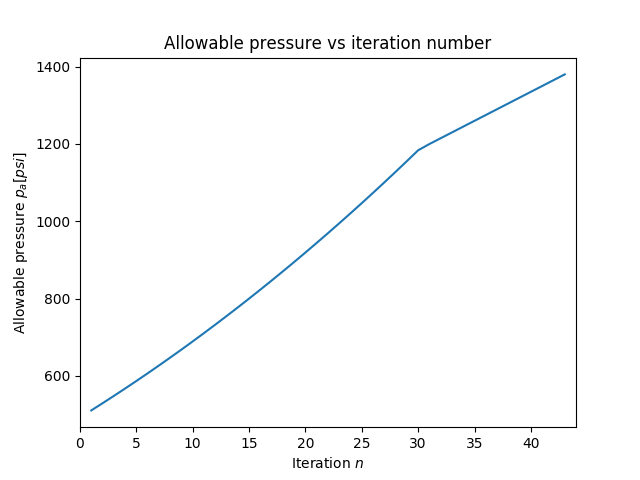
\includegraphics[scale=0.8]{2_vii2_cnvg}
	\caption{Convergence plot of $p_a$ using ASME's BPVC VIII-2.}
	\label{fig:2_vii2_cnvg}
\end{figure}

Convergence was reached at a thickness of $t = 23.4\ mm = 0.920\ in$ when $p_a\geq p_{req}$, after $n=43$ iterations. 


%%----------------------------------------------------------------------------------------------------------------------
\section{European Standard}
\subsection{EN-13445-3}
As per subsection 8.5.2.2 of \cite{EN134453}, the following procedure was used to calculate the required thickness $e_a$. Note that the script in Appendix~~\ref{appendix:a3} utilizes SI units as per \cite{EN134453}.

\begin{enumerate}
	\item Assume initial thickness value of $e_a$ and calculate $p_y$ with \ref{eq:2_EN_py}
	      \begin{equation}
	      	\label{eq:2_EN_py}
	      	p_y = \frac{\sigma_e e_a}{R}
	      \end{equation}
	\item Compute the lower failure pressure $p_m$ \ref{eq:2_EN_pm}, see 8.5.2.6 of \cite{EN134453} for $\varepsilon$
	      \begin{equation}
	      	\label{eq:2_EN_pm}
	      	p_m = \frac{E e_a  \varepsilon}{R}
	      \end{equation}
	\item With the $p_m/p_y$ ratio, use Figure 8.5.5 of \cite{EN134453} to find equivalent $p_r/p_y$
	\item Rearrange for $p_r$ and calculate allowable pressure $p$ ith \ref{eq:2_EN_pa}
	      \begin{equation}
	      	\label{eq:2_EN_pa}
	      	p = \frac{p_r}{S}
	      \end{equation}
	\item Check if $p \geq p_{req}$ as calculated from \ref{eq:2_preq}, if not, increase $e_a$ and go to Step 2\\
\end{enumerate}

Again, with the respective Python Script in Appendix~\ref{appendix:a3}, a convergence plot was created (see Figure~\ref{fig:2_en13445_cnvg}).
\begin{figure}[H]
	\centering
	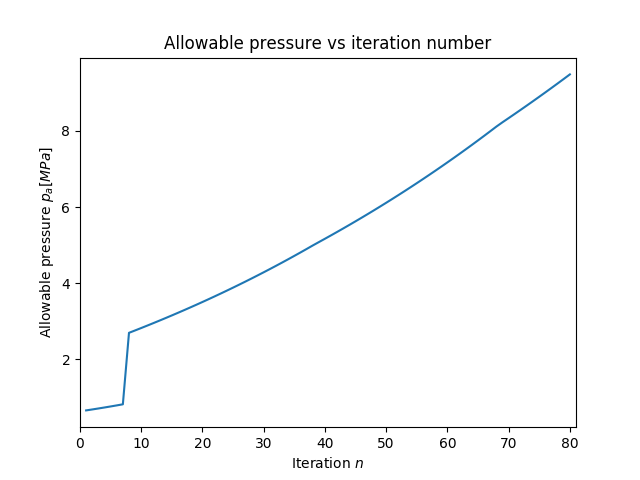
\includegraphics[scale=0.8]{2_en13445_cnvg}
	\caption{Convergence plot of $p_a$ using EN 13445-3.}
	\label{fig:2_en13445_cnvg}
\end{figure}

The script converged at thickness of $e_a = 32.8\ mm = 1.290\ in$ and an allowable pressure of $p\geq p_{req}$ after $n=80$ iterations. 

%%----------------------------------------------------------------------------------------------------------------------
\section{DNV}

\subsection{DNV-OS-D101}

As per \cite{DNVOSD101}, in subsection F215, Equation~\ref{eq:2_DNV_hoop} is presented as follows.

\begin{equation}
	\label{eq:2_DNV_hoop}
	\sigma_h = C\cdot\frac{T}{d_{thr}t}
\end{equation}

In this equation, $C$ is a factor based on the number of wraps on the drum,. for two layers $C=1.75$ \cite{DNVOSD101}. There are a few exceptions with this equation and they are listed as follows.

\begin{enumerate}
	\item The hoop stress $\sigma_h$ is limited to $\sigma_h \leq 0.85\cdot S_y$
	\item The calculated $\sigma_h$  if superseded with larger tested value\\
\end{enumerate}

Rearranging Equation~\ref{eq:2_DNV_hoop} for $t$, setting $\sigma_h = S_{allow}=S_y/SF$ (see Table~\ref{table:prelim_params}) and solving accordingly will yield a valid value of $t = 36.6\ mm = 1.440 \ in$. 

%----------------------------------------------------------------------------------------------------------------------
\section{TWPV Hoop Stress}

Using the well known hoop stress equation \cite{roarks} for a TWPV, Equation~\ref{eq:2_hoop} is presented as follows.

\begin{equation}
	\label{eq:2_hoop}
	\sigma_h = \frac{pR}{t}
\end{equation}

Again, rearranging for $t$ , $\sigma_h = S_{allow}=S_y/SF$ and using the pressure $p$ calculated in \ref{eq:2_preq}, solving accordingly will yield a valid value of $t = 21.0\ mm = 0.825 \ in$. Note that $\because R/t = 17 \geq 10$, the assumption of a TWPV is valid.

%%----------------------------------------------------------------------------------------------------------------------
\section{Comparison}

Based on the above sections, the results are summarized in Table~\ref{table:2_comp}.
\begin{table}[H]
	\centering
	\caption{Comparison $t$ according to method used.}
	\begin{tabular}{lccc}
		\textbf{Method}  & \textbf{$\mathbf{mm}$} & \textbf{$\mathbf{in}$} & \textbf{SF} \\
		\midrule
		ASME BPVC VIII-1 & $43.7$                 & $1.680$                & $1.5$       \\
		ASME BPVC VIII-2 & $23.4$                 & $0.920$                & $1.5$       \\
		EN 13445-3       & $32.8$                 & $1.290$                & $1.5$       \\    
		DNV-OS-D101      & $36.6$                 & $1.440$                & $1.5$       \\
		TWPV Hoop Stress & $21.0$                 & $0.825$                & $1.5$       \\
	\end{tabular}%
	\label{table:2_comp}%
\end{table}%

Based on these results the following observations may be made

\begin{itemize}
	\item ASME's BPVC VIII-1 is the most conservative
	\item TWPV Hoop Stress and ASME's BPVC VIII-2 yield the least conservative results
	\item Both EN 13445-3  and DNV-OS-D101 are somewhere in between \\
\end{itemize}

Now that there is a benchmark for the expected values, a more analytically approach will be taken in the following section.

%-----------------------------------------------------------------------------------------------------------------
%% Section3 : Preliminary Analysis
\chapter{Advanced Analysis}
	\label{chapt:prelim}

In this foregoing section, methods used to set up the analytical approach are discussed in detail. Please note that all parameters used in this section will follow Table~\ref{table:prelim_params}.

%----------------------------------------------------------------------------------------------------------------------
\section{Deflection \& Differential Relations}

The first key equation to setting up the differential relations is taken from \cite{nisbett2014shigley}. Equation~\ref{eq:Mcurve} shows the relationship between internal bending moment on a beam and its radius of curvature. 

\begin{equation}
	\label{eq:Mcurve}
	\frac{1}{\rho}=\frac{M}{EI}
\end{equation}

Where $1/\rho$ is the radius of curvature defined as Equation~\ref{eq:curve} \cite{nisbett2014shigley}. Note that for a small differential, the denominator approaches unity, leaving the final result.

\begin{equation}
	\label{eq:curve}
	\frac{1}{\rho}=\frac{d^2y/dx^2}{\left( 1 +(dy/dx)^2 \right)^\frac{3}{2}} \approx \frac{d^2y}{dx^2}
\end{equation}

From Equation~\ref{eq:curve} deflection $y(x)$ relations for slope \ref{eq:slope}, moment \ref{eq:mmt} and shearing force \ref{eq:shr} as a consequence \cite{nisbett2014shigley}.

\begin{equation}
	\label{eq:slope}
	\theta(x) = \frac{dy}{dx}
\end{equation}

\begin{equation}
	\label{eq:mmt}
	M(x) = EI\ \frac{d\theta(x)}{dx} = EI\ \frac{d^2y}{dx^2}
\end{equation}

\begin{equation}
	\label{eq:shr}
	V(x) = \frac{dM(x)}{dx} = EI\ \frac{d^3y}{dx^3}
\end{equation}

The above listed equations are important for understand how deflection translates to other internal loading.\\

Furthermore, boundary conditions (BC) may be derived as a result. The following equations assume that the boundary in question is located at $x_0$.\\

\textbf{Free Ends:} no loading, allowed to deform\\
\begin{equation}
	\label{eq:2_freeBC}
	\begin{aligned}
		y(x_0) = y_0          \\
		\theta(x_0)= \theta_0 \\
		M(x_0) = 0            \\
		V(x_0) = 0            
	\end{aligned}
\end{equation}

\textbf{Simply Supported:} free to rotate\\
\begin{equation}
	\label{eq:2_endBC}
	\begin{aligned}
		y(x_0)= 0            \\
		\theta(x_0)=\theta_0 \\
		M(x_0)= 0            \\
		V(x_0) =V_0          
	\end{aligned}
\end{equation}

\textbf{Fixed:} load is carried at the ends\\
\begin{equation}
	\label{eq:2_fixedBC}
	\begin{aligned}
		y(x_0)=0      \\
		\theta(x_0)=0 \\
		M(x_0)=M_0    \\
		V(x_0) =V_0   
	\end{aligned}
\end{equation}

The equations from this subsection serve as an important set up for the more complex approach derived in the following section. 

%----------------------------------------------------------------------------------------------------------------------
\section{Theory of Cylindrical Shells}
\label{section:3_shells}

As per \cite{timoshenko1959theory}, this section covers the method of approximating the drum barrel as a long thin cylindrical shell. With this assumption, the governing ordinary differential equation (ODE) is derived. First, the following coordinate system is presented as per Figure~\ref{fig:CoordSyst} below. Note that all symbols and steps in this subsquent derivation will follow \cite{timoshenko1959theory}.

\begin{figure}[H]
	\centering
	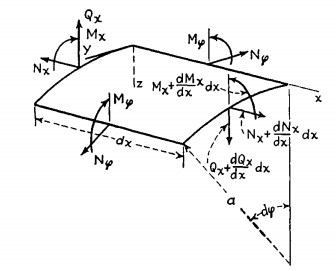
\includegraphics[width=0.6\textwidth]{CoordSyst}
	\caption[Coordinate system adopted for derivation of ODE.]{Coordinate system adopted for derivation of ODE.\protect\cite{timoshenko1959theory}}
	\label{fig:CoordSyst}
\end{figure}

From the above figure, the differential area of the cylindrical shell is presented as Equation~\ref{eq:diffsurf}. Note that in the foregoing section, $x$ is the axial direction, $a$ is the shell's outer radius and $\varphi$ is the circumferential direction.
 
\begin{equation}
	\label{eq:diffsurf}
	dA = dS\ dx = a\ d\varphi \ dx   
\end{equation}

Equilibrium is performed as a force balance in the $x, z$ axes and moment balance about the $y$ axis and presented as Equations ~\ref{eq:eqbrm_x}, ~\ref{eq:eqbrm_z}, ~\ref{eq:eqbrm_y} respectively. Note that $Z$ denotes and external pressure applied to the shell (not shown in Figure~\ref{fig:CoordSyst}).

\begin{equation}
	\label{eq:eqbrm_x}
	\frac{dN_x}{dx}\ a\ d\varphi \ dx = 0
\end{equation}

\begin{equation}
	\label{eq:eqbrm_z}
	\frac{dQ_x}{dx}\ a\ d\varphi \ dx+ N_\varphi \ a\ d\varphi \ dx +Z\ a\ d\varphi \ dx= 0
\end{equation}

\begin{equation}
	\label{eq:eqbrm_y}
	\frac{dM_x}{dx}\ a\ d\varphi \ dx- Q_x\ a\ d\varphi \ dx= 0
\end{equation}

First looking at \ref{eq:eqbrm_x}, the axial force $N_x$ is determined by taking the integral with respect to $x$ \ref{eq:eqbrm_x2}. 

\begin{equation}
	\label{eq:eqbrm_x2}
	N_x = C = 0 
\end{equation}

The above equation states that the effects of bending due to the axial forces are neglected, which is a valid assumption for thin shells \cite{timoshenko1959theory}.\\

Similarly with \ref{eq:eqbrm_z} and \ref{eq:eqbrm_y}, simplifications will lead to \ref{eq:eqbrm_z2} and \ref{eq:eqbrm_y2} respectively.
\begin{equation}
	\label{eq:eqbrm_z2}
	\frac{dQ_x}{dx}+\frac{1}{a}\ N_\varphi = -Z
\end{equation}

\begin{equation}
	\label{eq:eqbrm_y2}
	\frac{dM_x}{dx}- Q_x= 0
\end{equation} 

Next, differential relations between displacement and strain are presented in Equation~\ref{eq:strain_xphi}. Note $u$ and $w$ are displacements in both $x$ and $z$ directions.

\begin{equation}
	\label{eq:strain_xphi}
	\begin{aligned}
		\varepsilon_x = \frac{du}{dx}      \\
		\varepsilon_\varphi = -\frac{w}{a} 
	\end{aligned}
\end{equation}

From Hooke's law $N_x$ may be also written as Equation~\ref{eq:Hookes_Nx}. Substituting Equation~\ref{eq:strain_xphi} will yield the following. Note that $h$ represents the thickness of the cylindrical shell.
\begin{equation}
	\label{eq:Hookes_Nx}
	N_x = \frac{Eh}{1-\nu^2}\ \left( \varepsilon_x + \nu \varepsilon_\varphi \right) =  \frac{Eh}{1-\nu^2}\ \left( \frac{du}{dx} -\nu \ \frac{w}{a} \right)
\end{equation} 

%%%%%%%%%%%%%%%%%%%%%%%%%%%%%%%%%%%%%%%%%%%%%%%%%
Solving Equation~\ref{eq:Hookes_Nx} using ~\ref{eq:eqbrm_x2} leaves \ref{eq:Nx_simpl}.
\begin{equation}
	\label{eq:Nx_simpl}
	\frac{du}{dx} =  \nu \ \frac{w}{a}
\end{equation} 

Similarly, with $N_\varphi$, again applying \ref{eq:strain_xphi} leaves \ref{eq:Nphi_simpl}.
\begin{equation}
	\label{eq:Hookes_Nphi}
	N_\varphi = \frac{Eh}{1-\nu^2}\ \left( \varepsilon_\varphi + \nu \varepsilon_x \right) = \frac{Eh}{1-\nu^2}\  \left( -\frac{w}{a}+\nu \ \frac{du}{dx} \right)
\end{equation} 

\begin{equation}
	\label{eq:Nphi_simpl}
	N_\varphi = - \frac{Ehw}{a}
\end{equation}

As a result of no change in curvature in the $\varphi$ direction, we know that $\frac{dM_\varphi}{d\varphi}= 0$ hence no change in the circumferential moments \cite{timoshenko1959theory}. This relation is translated to axial moments $M_x$ with \ref{eq:Mphix}.

\begin{equation}
	\label{eq:Mphix}
	\begin{aligned}
		M_\varphi = \nu M_x        \\
		M_x = -D \frac{d^2w}{dx^2} 
	\end{aligned}
\end{equation}

Where $D$ is defined as the flexural rigidity of the shell \ref{eq:flexrig}. This term replaces the $EI$ term from Equations~\ref{eq:Mcurve} - \ref{eq:shr}.

\begin{equation}
	\label{eq:flexrig}
	D \triangleq \frac{Eh^3}{12(1-\nu^3)}
\end{equation}

Simplifying \ref{eq:eqbrm_z2} to get $Q_x = \frac{dM_x}{dx}$, the following is put in \ref{eq:eqbrm_y2} to get the final ODE in Equation~\ref{eq:de1}

\begin{equation}
	\label{eq:de1}
	\begin{aligned}
		\frac{d^2M_x}{dx^2}+\frac{1}{a} \ N_\varphi = -Z \\
		D\ \frac{d^4w}{dx^4}+\frac{Eh}{a^2} \ w = Z      \\
		\frac{d^4w}{dx^4}+\beta^4 \ w = \frac{Z}{D}      
	\end{aligned}
\end{equation} 

Where $\beta^4$ is some parameter defined as \ref{eq:betaquad}.

\begin{equation}
	\label{eq:betaquad}
	\beta^4 \triangleq \frac{Eh}{4a^2D}= \frac{3(1-\nu^2)}{a^2h^2}
\end{equation}

The solution to this common fourth order, linear, non-homogeneous, ODE in \ref{eq:de1} has a general solution of Equation~\ref{eq:solnDE} \cite{timoshenko1959theory}.

\begin{equation}
	\label{eq:solnDE}
	w(x)=e^{\beta x} \left(C_1 \cos \beta x +C_2 \sin \beta x \right)+e^{-\beta x} \left(C_3 \cos \beta x +C_4 \sin \beta x \right) +f(x)
\end{equation}

Where $ C_1, C_2, C_3, C_4$ are integration constants to be solved based on BC and $f(x)$ is the particular solution to the ODE (recall $y_{general}=y_{homogeneous}+y_{particular}$).\\

In the following section, a specific solution of this differential equation will be determined.

%----------------------------------------------------------------------------------------------------------------------

\section{Roark's Solution}
\label{section:3_roark}

The previous equation prepared the set up to the solution procedure outlined in Example 3 of Chapter 12, p.538 \cite{roarks}. A similar solution was developped in an Excel \cite{EXCEL} calculator (see Appendix B).The main important factor lies in the assumptions of a long shell(i.e. $\beta l \geq 6$) and a TWPV (i.e $R/t \geq 10$).\\

Referring to Appendix B, a final calculated value of $t=1.686 \Unit{in}= 42.8 \Unit{mm}$ upon confirming the assumptions.

\section{Roark's Buckling}
\label{section:3_buckle}

Up to this point, all values for calculating the drum barrel thickness have focused on the stress state. It was proposed by John Umina to investigate buckling. To confirm that stress is primary mode of failure, a linear buckling analysis is completed.\\

With equations from Table 35 of \cite{roarks}, the following relations are presented. First, Equation~\ref{eq:3_buckle1} is presented for a long thin tube under uniform external pressure with ends simply supported.
\begin{equation}
	\label{eq:3_buckle1}
	p' =\frac{1}{4} \frac{E}{1-\nu^2} \frac{t^3}{R^3}
\end{equation}

To classify as a long tube, the length of the barrel $L$ must be greater the critical length as calculated with Equation~\ref{eq:3_lcrit}.
\begin{equation}
	\label{eq:3_lcrit}
	L' = 4.90 R \sqrt{\frac{R}{t}}
\end{equation}

For the studied range of $t \in [0.05, 1.05] \Rightarrow L < L' \therefore$ Equation~\ref{eq:3_buckle2} must is to calculate the critical buckling pressure for a short thin cylinder.

\begin{equation}
	\label{eq:3_buckle2}
	p' =0.807\  \frac{Et^2}{LR}\  \sqrt[4]{\left( \frac{1}{1-\nu^2} \right)^3 \left( \frac{t}{R}\right)^2}
\end{equation}

With \ref{eq:3_buckle2} and the aforementioned thickness range, critical pressure values were computed with the \cite{PYTHON} script in Appendix~\ref{appendix:a4}. These results are displayed in the following plot (see Figure~\ref{fig:3_buckling}).

\begin{figure}[H]
	\centering
	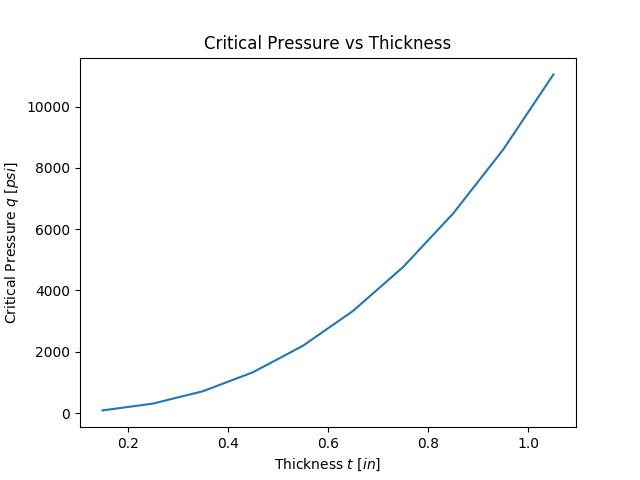
\includegraphics[scale=0.75]{3_buckling}
	\caption{Variation of critical buckling pressure $p'$ with $t$.}
	\label{fig:3_buckling}
\end{figure}

As depicted in the above figure, a very low thickness is required to achieve a critical buckling pressure $p'$ of $137\Unit{psi} \/\ 9.484\Unit{MPa}$ (as per Equation~\ref{eq:2_preq}).\\

By rearranging, \ref{eq:3_buckle2} for $t$ and setting $p'=1376\Unit{psi}$, a critical thickness of $0.418\Unit{in}= 10.6\Unit{mm}$ is required to avoid buckling. Based on these conclusions, buckling will not be the primary failure mode for the drum barrel given the loading scenario. The following section will validate all conclusions with a series of FEA simulations.





%-----------------------------------------------------------------------------------------------------------------
%% Section 4 : Finite Element Analysis
\chapter{Finite Element Analysis}
	This section uses ANSYS Mechanical FEA software \cite{ANSYS} to validate analytical findings from previous sections. Please note that all results presented in the foregoing section focuses on USC units however, important results will be converted to their respective SI units. The overall ANSYS geometry is first presented followed by a series of FEA runs which are summarized below (see Table~\ref{table:4_runs}).

\begin{table}[H]
  \centering
  \caption{Labeling of FEA runs.}
    \begin{tabular}{cll}
    \textbf{Run} & \textbf{Focus} & \textbf{Description}\\
    \hline
    1A    & Drum Stress & Fixed ends, uniform $p$\\
    1B    & Drum Stress & Simply supported ends, uniform $p$ \\
    2A    & Drum Stress & Fixed ends, Capstan $p, z=24.5$, various $\mu$ \\
    2B    & Drum Stress & Simply supported ends, Capstan $p, z=24.5$, various $\mu$ \\
    2C    & Drum Stress & Fixed ends, Capstan $p, z=0$, various $\mu$ \\
    2D    & Drum Stress & Simply supported ends, Capstan $p, z=0$, various $\mu$ \\
    3     & Drum Buckling & Simply supported ends, uniform $p$ \\
    4     & Flange Stress & Fixed ends, uniform $p$ \\
    \end{tabular}%
  \label{table:4_runs}%
\end{table}%


\section{Model}

Both $D$ and $L$ parameters from Table~\ref{table:prelim_params} are used to model the drum barrel's geometry. This model utilizes a thin cylindrical surface with inwards parameterized thickness to save computational time. A series of parametric studies will be performed determine how maximum stresses vary with $t$. Note that flanges are not shown in this model as they will be added in the final run. The thin surface also allows for a simple initial ANSYS generated coarse mesh. The preliminary geometry, coordinate system and mesh adopted in the foregoing analysis is shown below in Figure~\ref{fig:4_mesh}.

\begin{figure}[H]
	\centering
	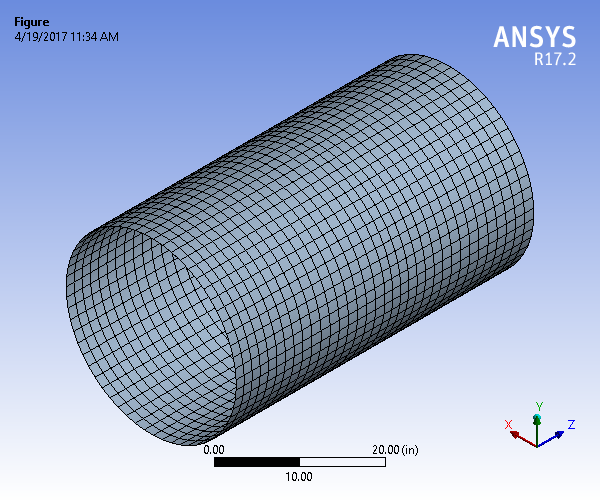
\includegraphics[scale=0.4]{4_mesh}
	\caption{Initial model geometry, coordinate system and coarse mesh.}
	\label{fig:4_mesh}
\end{figure}

Numerical accuracy of results will be assured by performing mesh refinement when possible in all foregoing simulations.

\section{Run 1: Uniform Pressure}
\label{section:4_R1}

The first FEA run will explore the uniform externally pressurized drum with both fixed and simply supported ends. 

\subsection{Boundary Conditions}
\label{subsection:R1BC}

An initial simulation will be performed with fixed ends (BC as per Equation~\ref{eq:2_fixedBC}) and $t=0.500\Unit{in}$. Figure~\ref{fig:4_R1_p} shows the uniform external pressure of $1376 \Unit{psi}$ or $9.484 \Unit{MPa}$ as per \ref{eq:2_preq}.
\begin{figure}[H]
	\centering
	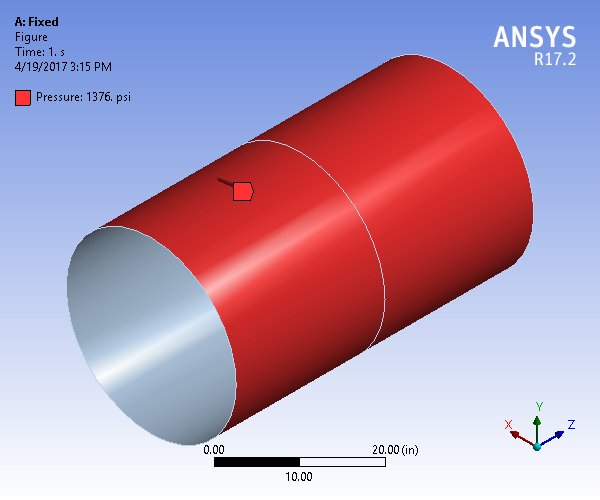
\includegraphics[scale=0.4]{4_R1_p}
	\caption{Uniform external pressure on model.}
	\label{fig:4_R1_p}
\end{figure}

\subsection{Results}

A mesh refinement is completed and yields the equivalent maximum stress results in Figure~\ref{fig:4_R1_stress} below. Note results are shown for $t=0.500\Unit{in}$.

\begin{figure}[H]
	\centering
	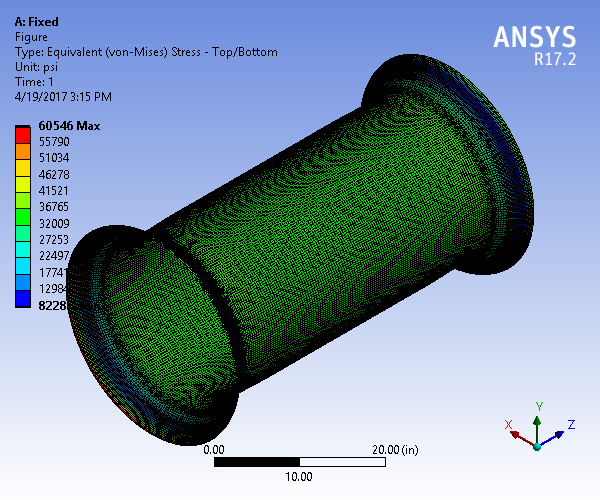
\includegraphics[scale=0.4]{4_R1_stress}
	\caption{Maximum equivalent stress results for Run 1.}
	\label{fig:4_R1_stress}
\end{figure}

It is apparent from the above figure that the fixed ends are carrying most of load. In hopes of better understanding how this uniform pressure results in stress, a parametric study is performed by varying the drum thickness $t$ for a cylinder with both fixed and simply supported ends.

\subsection{Parametric Study}

A parametric study is performed with a range of $t \in [0.500, 1.750]$ for both fixed and simply supported ends. The results from this simulation are shown below in Figure~\ref{fig:4_R1_sweep} \cite{EXCEL}. The allowable stress limit of $23,333 \Unit{psi}$ (Equation~\ref{eq:2_sigall}) is also shown for reference.

\begin{figure}[H]
	\centering
	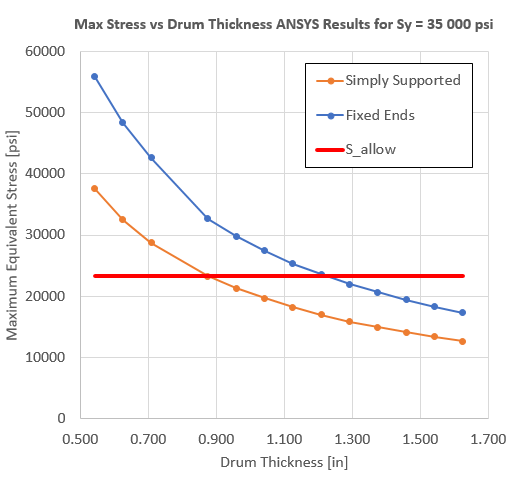
\includegraphics[scale=0.65]{4_R1_sweep}
	\caption{Results the parametric sweep for Run 1.}
	\label{fig:4_R1_sweep}
\end{figure}

From the above plot, thicknesses of $1.250 \Unit{in}$ and $0.875\Unit{in}$ are required for a uniformly loaded cylinder with fixed (Run 1A) and simply supported ends (Run 1B), respectively. These results are relatively close to their analytical counterparts. Several sources of error could be the reason for discrepancies, those of which will be further discussed in Section~\ref{subsection:5_numerr}.

\section{Run 2: Capstan Pressure}
\label{section:4_R2}
The second run elaborates on the results determined from Run 1. The aim of Run 2 is to determine how the decaying Capstan pressures translates to stress. This pressure profile represents a more realistic loading scenario.

\subsection{Boundary Conditions}

Initial results are shown for simply supported ends (i.e. BC as per Equation~\ref{eq:2_endBC} ) and a thickness of $0.500$ in.\\

The variable Capstan pressure is shown applied to the external surface of the cylinder in Figure~\ref{fig:4_R2_pvar}. This pressure profile is also shown in Figure~\ref{fig:4_R2_pvarplot} as per the results in Section~\ref{subsection:alt}. Note that the pressure profile is shown for $\mu=0.05$, the worst-case scenario. It is also applied beginning at the center of the drum or at $z=24.5$.

\begin{figure}[H]
	\centering
	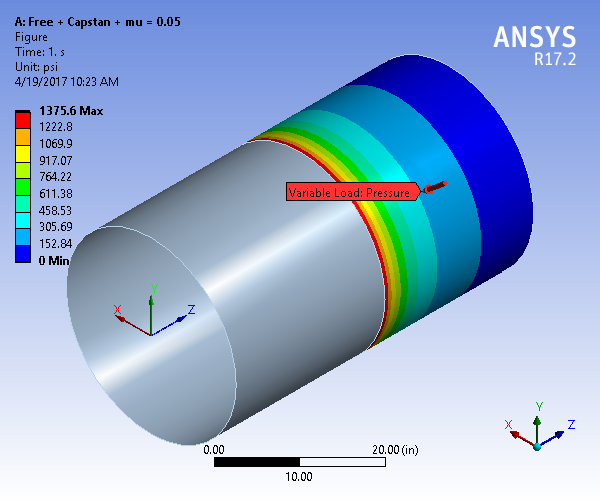
\includegraphics[scale=0.4]{4_R2_pvar}
	\caption{Variable Capstan pressure for $\mu=0.05$ at $z=24.5$.}
	\label{fig:4_R2_pvar}
\end{figure}
\begin{figure}[H]
	\centering
	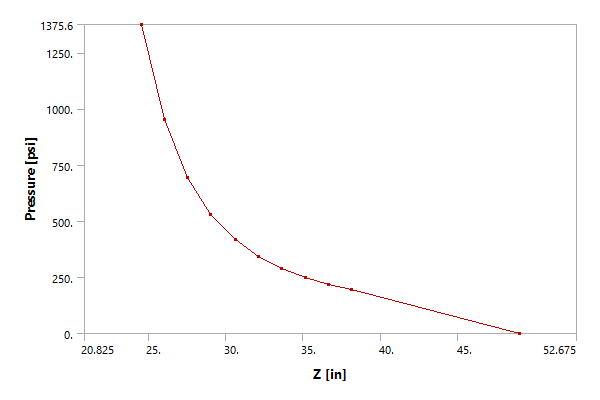
\includegraphics[scale=0.5]{4_R2_pvarplot}
	\caption{Variable Capstan pressure $p(z)$.}
	\label{fig:4_R2_pvarplot}
\end{figure}

Again, note from above that $p(24.5)=1376$ psi.

\subsection{Results}

Total deformation results are shown below in Figure~\ref{fig:4_R2_def_mu05}. The maximum deformation seen along the $z$ axis in the $y$ direction is also shown in Figure~\ref{fig:4_R2_topdefplotmu05}.

\begin{figure}[H]
	\centering
 	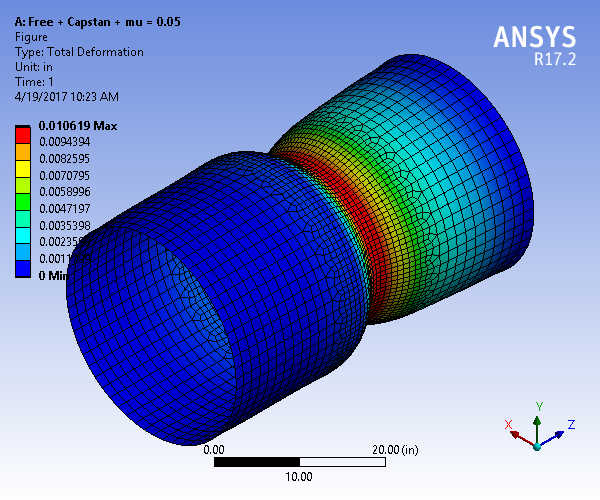
\includegraphics[scale=0.4]{4_R2_def_mu05}
 	\caption{Total deformation results for Run 2.}
 	\label{fig:4_R2_def_mu05}
 \end{figure}
 
 \begin{figure}[H]
 	\centering
 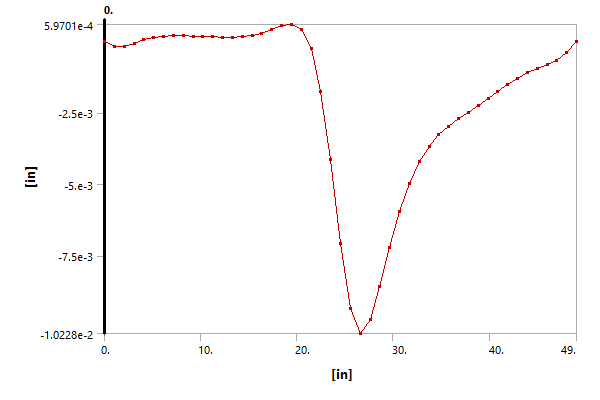
\includegraphics[scale=0.5]{4_R2_topdefplotmu05}
 	\caption{Total deformation in $y$ as a function of $z$.}
 	\label{fig:4_R2_topdefplotmu05}
 \end{figure}
 
Referring to Table~\ref{table:3_beta} for $t=0.500 \therefore \beta = 0.486 \Rightarrow x= 24.500+12.345 = 37.7$ in for $\beta x \geq 6$. From the above deformation plot, it can be observed that at $x=z=37.7$, deformation is nearly zero however loading is not technically zero at this point (see Figure~\ref{fig:4_R2_pvarplot}). These observations follow those from long shell theory.\\

The maximum stress results are shown in Figure~\ref{fig:4_R2_stress_mu05} below for Run 2.

\begin{figure}[H]
	\centering
	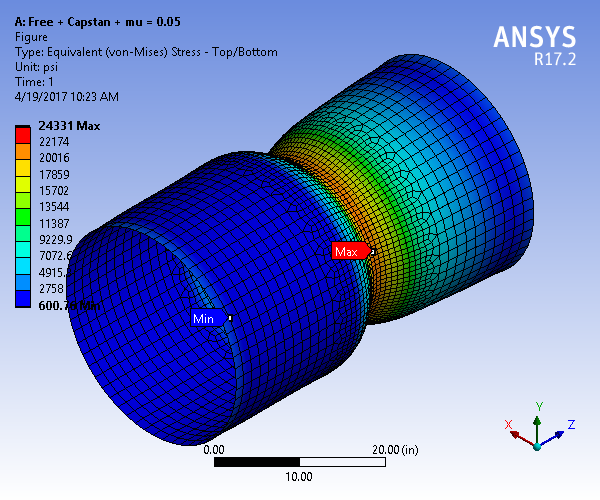
\includegraphics[scale=0.4]{4_R2_stress_mu05}
	\caption{Maximum equivalent stress results for Run 2.}
	\label{fig:4_R2_stress_mu05}
\end{figure}

Unlike the results from Run 1, it appears that the maximum stress occurs after slightly after the location where pressure is maximum. The maximum stress is also much lower. This behavior is next explored.

\subsection{Parametric Study}

With a range of $t\in [0.15, 1.05]$, and pressure profiles for $\mu =0.05, 0.50$, maximum stress is calculated for a cylinder with both fixed and simply supported ends. The sweep results are shown below in Figure~\ref{fig:4_R2_sweep} \cite{EXCEL}.  The allowable stress limit is also shown.

\begin{figure}[H]
	\centering
	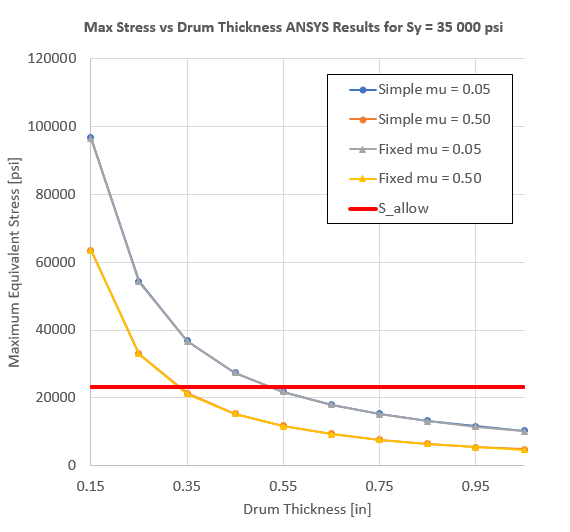
\includegraphics[scale=0.65]{4_R2_sweep_FE_SSE}
	\caption{Results of parametric study for FEA Run 2A-B.}
	\label{fig:4_R2_sweep}
\end{figure}

The main observation from the above sweep summary is that for a Capstan pressure profile beginning at the center of the drum ($z=24.5$), maximum stress is not dependent on the end conditions. This observation can be validated through thin shell theory (i.e $\beta x \geq 6$) which dictates that internal loadings disappear once a certain distance from the point of load application is reached.\\

From the above plot, it appears that a thickness of $t \geq 0.55 \Unit{in}$ would appear to be sufficient for both fixed (Run 2A) and simply supported ends (Run 2B).\\

To investigate end conditions effects, the Capstan pressure is applied from $0 \leq z \leq 24.5$ (see Figure~\ref{fig:4_R2_BC_c}). The results for $t=0.500$ and $\mu=0.05$ with simply supported ends are shown in Figure~\ref{fig:4_R2_stress_c} for reference.
\begin{figure}[H]
	\centering
	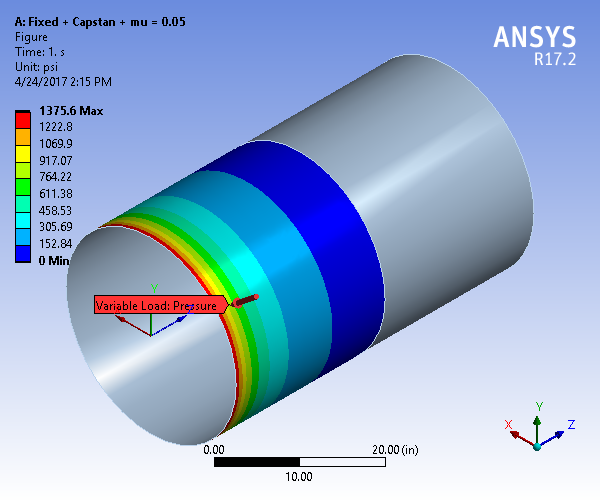
\includegraphics[scale=0.4]{4_R2_BC_c}
	\caption{Variable Capstan pressure.}
	\label{fig:4_R2_BC_c}
\end{figure}

\begin{figure}[H]
	\centering
	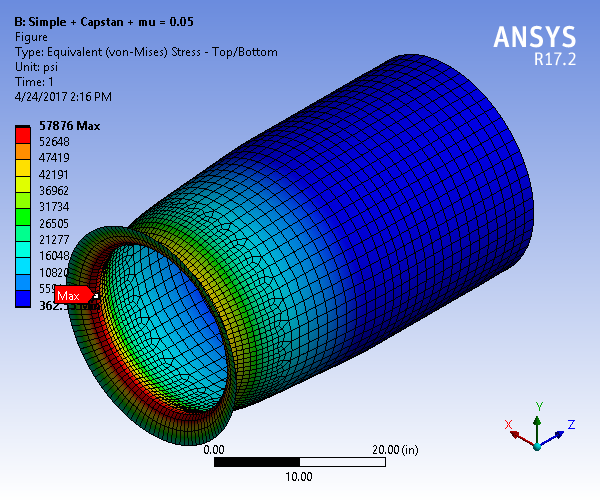
\includegraphics[scale=0.4]{4_R2_stress_c}
	\caption{Total stress results.}
	\label{fig:4_R2_stress_c}
\end{figure}

From this, a similar sweep was performed with the same aforementioned range and loading scenario (see Figure~\ref{fig:4_R2_sweep2}).

\begin{figure}[H]
	\centering
	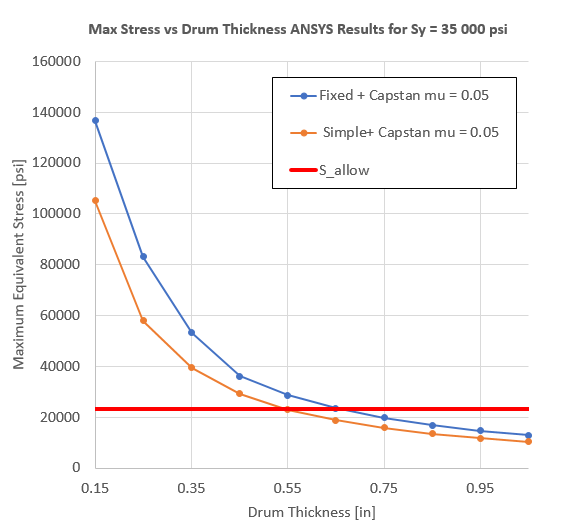
\includegraphics[scale=0.65]{4_R2_sweep_c}
	\caption{Results of parametric study for FEA Run 2C-D.}
	\label{fig:4_R2_sweep2}
\end{figure}

Moving the initial location of the pressure load application from $z=24.5$ to $z=0$ yields required thicknesses of $0.650$ and $0.550$ in for fixed (Run 2C) and simply supported ends (Run 2D), respectively.

\section{Run 3: Eigenvalue Buckling}
\label{section:4_R3}

To validate the conclusion made from Section~\ref{section:3_buckle}, Run 3 focuses on performing a linear eigenvalue buckling analysis in ANSYS. The analysis is said to be linear as in ANSYS, it is coupled with a linear static structural analysis system (see Figure~\ref{fig:4_R3_wb}).

\begin{figure}[H]
	\centering
	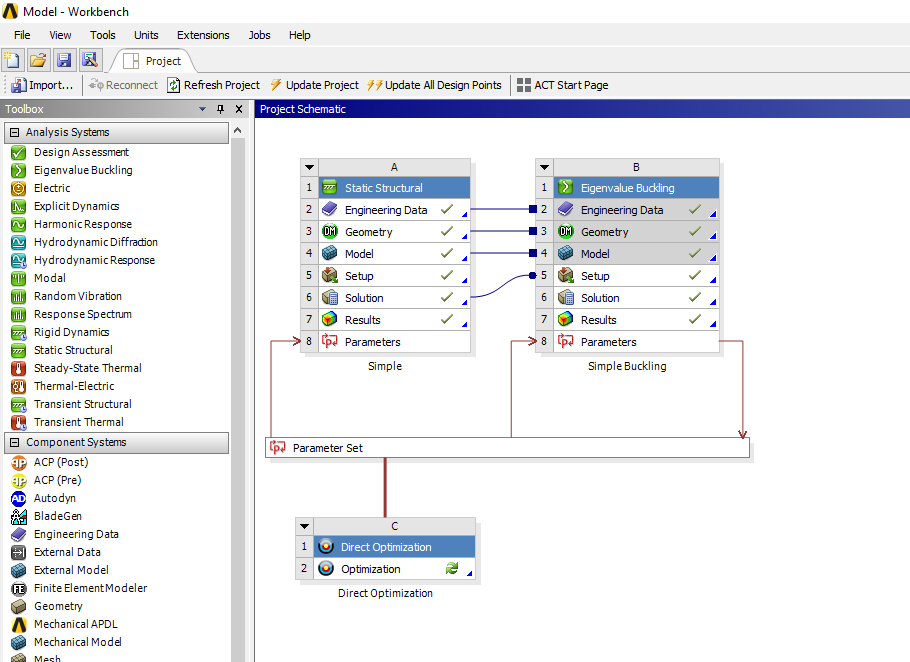
\includegraphics[scale=0.4]{4_R3_wb}
	\caption{ANSYS Workbench project schematic.}
	\label{fig:4_R3_wb}
\end{figure}

\subsection{Boundary Conditions}

ANSYS sets the linear static structural analysis system as the pre-stressed state and then performs the eigenvalue buckling analysis. From this, load factors $\lambda$ are returned. These factors are defined as Equation~\ref{eq:4_loadfactor} \cite{ANSYS}.
\begin{equation}
	\label{eq:4_loadfactor}
	p' = \lambda \ p_0
\end{equation}

The critical buckling pressure $p'$ based on the pre-stressed state is simply a multiplier $\lambda$ of the applied load $p_0$. For this reason, a uniform unit load pressure of $p_0 = 1\Unit{psi}$ is applied in the coupled static structural system. Furthermore, the ends will be simply supported to match the BC from Section~\ref{section:3_buckle}.\\


With the ends simply supported (Equation~\ref{eq:2_endBC}), the unit pressure load is applied to external surface (see Figure~\ref{fig:4_R3_BC}). Also, for comparison of critical buckling calculations in Section~\ref{section:3_buckle}, a thickness of $t=0.418\Unit{in}$ is used in the foregoing results. 

\begin{figure}[H]
	\centering
	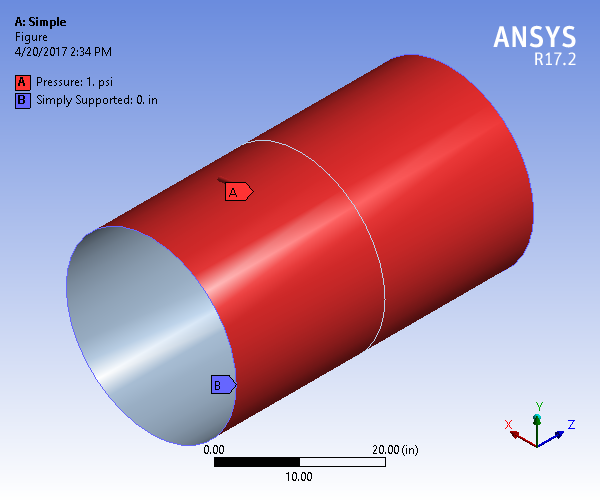
\includegraphics[scale=0.4]{4_R3_BC}
	\caption{Eigenvalue buckling analysis BC.}
	\label{fig:4_R3_BC}
\end{figure}

\subsection{Results}

Unfortunately, ANSYS is unable to perform a mesh refinement study for a coupled system analysis hence, an initial extra fine mesh is used to assure numerically accurate results on the first iteration. Results are shown below (see Figure~\ref{fig:4_R3_mode1}) for the first eigenvalue or mode $\psi = 1$.
\begin{figure}[H]
	\centering
	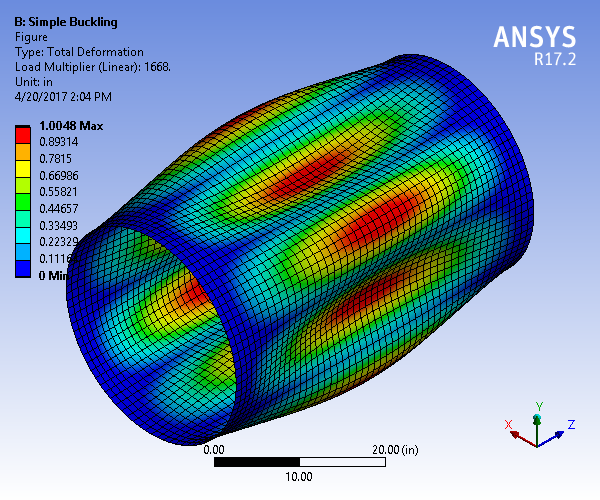
\includegraphics[scale=0.4]{4_R3_mode1}
	\caption{Total deformation results for mode $\psi = 1$.}
	\label{fig:4_R3_mode1}
\end{figure}

From above, a load factor of $\lambda = 1668$ is calculated for $t= 0.418\Unit{in}$. This value is within about $21.2\%$ of the expected analytical results of Section~\ref{section:3_buckle}, which is a reasonable margin for a first iteration. Note that the above results do not represent actual displacements but simply to visualize how the cylinder would deform when excited to the first mode \cite{ANSYS}.

\subsection{Parametric Study}

Again for $t\in [0.05, 1.05]$, a parametric study is performed. Results for the first, fifth and tenth mode (i.e. $\psi = 1, 5, 10$) are plotted against the thickness range of interest in Figure~\ref{fig:4_R3_modesweep} below, as per \cite{PYTHON} script in Appendix~\ref{appendix:a4}. The required pressure of $p =1376\Unit{psi}$ is also shown for reference in Figure~\ref{fig:4_R3_comp} where analytical and FEA results are compared.

\begin{figure}[H]
	\centering
	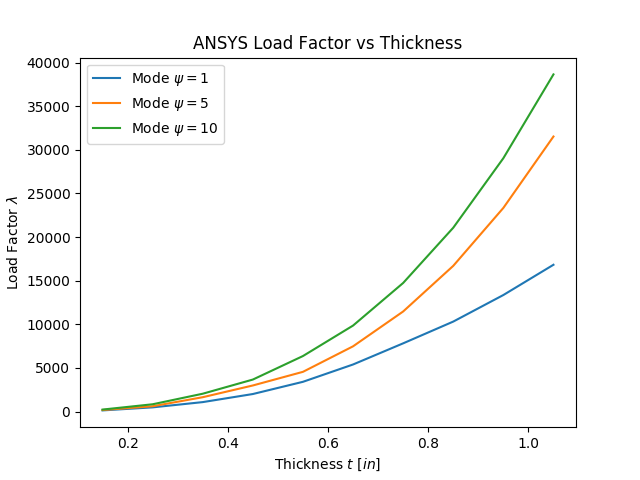
\includegraphics[scale=0.65]{4_R3_modesweep}
	\caption{Parametric sweep results for various $t, \psi$.}
	\label{fig:4_R3_modesweep}
\end{figure}

\begin{figure}[H]
	\centering
	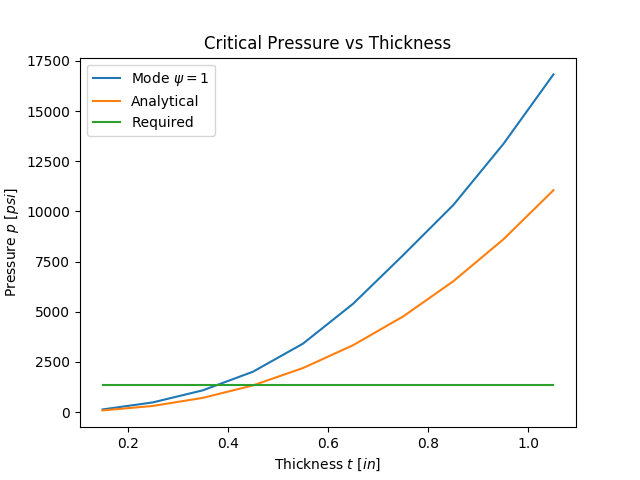
\includegraphics[scale=0.65]{4_R3_comp}
	\caption{Comparison of analytical and FEA results.}
	\label{fig:4_R3_comp}
\end{figure}

Focusing on the buckling mode of interest (i.e. $\psi=1$), observations from the above plots confirms the conclusion from Section~\ref{section:3_buckle} that failure by stress will occur before buckling. If anything, FEA results show that the analytical results previously calculated are more conservative however, this could likely be attributed to the numerical error as previously discussed.\\

The FEA Run 3 shows that to achieve a critical buckling pressure of $p'=p_{req}$, a thickness of $t=0.375\Unit{in}=9.5\Unit{mm}$ is sufficient.

\section{Run 4: Flanges}
\label{section:4_R4}
Due to time constraints, Run 4 serves as a preliminary benchmark for sizing the thickness of a 36 in OD flange. This foregoing FEA run utilizes a constant barrel $t=0.625\Unit{in}$.\\

Expanding on the thin cylindrical geometry from Figure~\ref{fig:4_mesh}, circular flanges are added to each end, also modeled as thin surfaces with parameterized thickness. Figure~\ref{fig:4_R4_mesh} below shows the mesh for the modeled assembly. An initial fine mesh  is used again as convergence for numerical precision is not possible for assemblies in ANSYS.
\begin{figure}[H]
	\centering
	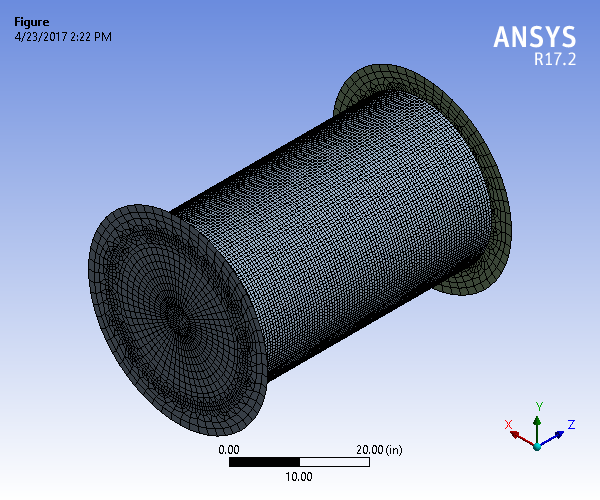
\includegraphics[scale=0.4]{4_R4_mesh}
	\caption{Drum assembly fine mesh.}
	\label{fig:4_R4_mesh}
\end{figure}

\subsection{Boundary Conditions}

The worst-case flange loading is explored by applying uniform external pressure of 1376 psi on the drum. Also, the circumference of a 5 in OD circular region is held fixed to model the winch shafts (see Figure~\ref{fig:4_R4_BC}).
\begin{figure}[H]
	\centering
	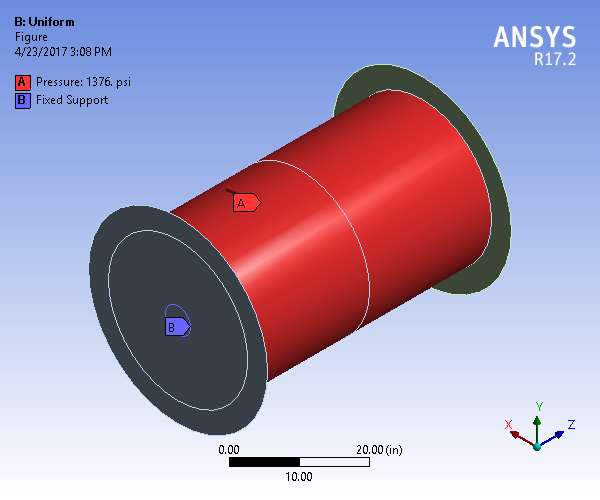
\includegraphics[scale=0.4]{4_R4_BC}
	\caption{Uniform external pressure and fixed shaft flange region.}
	\label{fig:4_R4_BC}
\end{figure}

\subsection{Results}

Both maximum stress of entire assembly (see Figure~\ref{fig:4_R4_res2}) and single flange (see Figure~\ref{fig:4_R4_res1}) are shown below. Note these results are for 0.125 in thick flanges.

\begin{figure}[H]
	\centering
	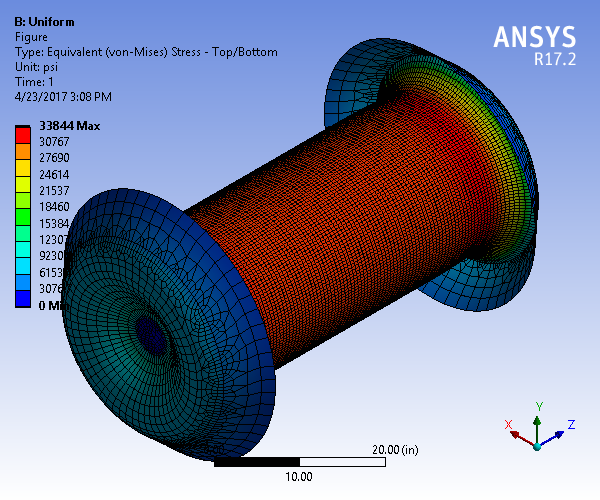
\includegraphics[scale=0.4]{4_R4_res2}
	\caption{Drum assembly stress results.}
	\label{fig:4_R4_res2}
\end{figure}
\begin{figure}[H]
	\centering
	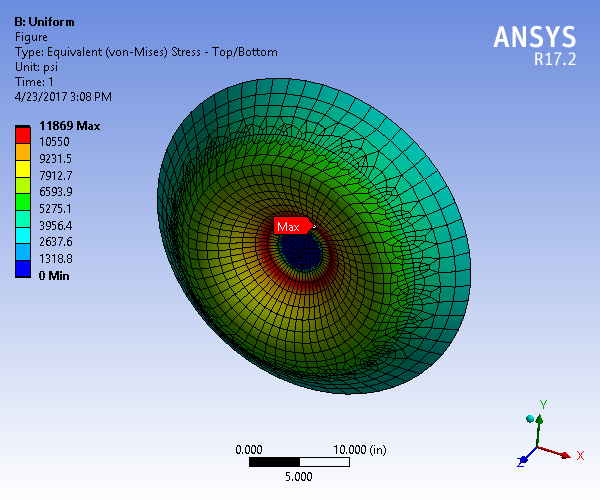
\includegraphics[scale=0.4]{4_R4_res1}
	\caption{Flange stress results for $t=0.125 \Unit{in}$.}
	\label{fig:4_R4_res1}
\end{figure}

The first observation from these above plots is that the drum barrel will experience the highest stress state.\\

Next, based on the stress results shown for the shaft side of the flange, maximum stress is exhibited near the perimeter of the 5 in OD fixed circular region. It must be noted however that even for a relatively thin flange (0.125 in) the maximum stress is still reaches about half ($\approx 50.8\%$) of the allowable limit.

\subsection{Parametric Study}

The final parametric study of this section explores flanges thicknesses $\in [0.063, 1.000]$. Results for both uniform and worst-case Capstan pressure profile ($\mu=0.05$) are simulated for comparion. The results are shown below in Figure~\ref{fig:4_R4_sweep} \cite{EXCEL}.

\begin{figure}[H]
	\centering
	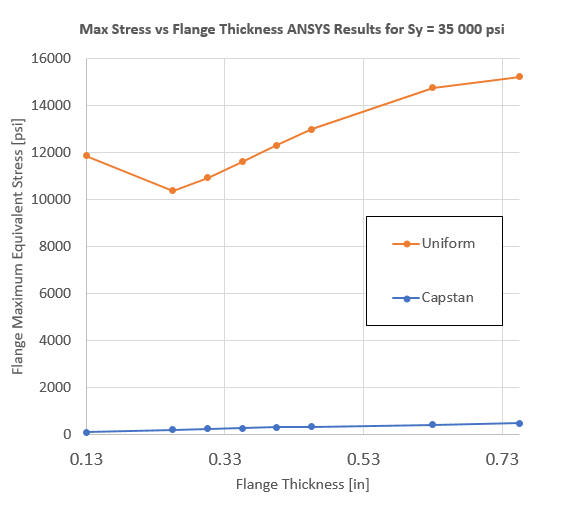
\includegraphics[scale=0.65]{4_R4_sweep}
	\caption{Results of parametric study for FEA Run 4.}
	\label{fig:4_R4_sweep}
\end{figure}

At first glance, the above sweep results do not appear to be relevant however after much discussion with both John Umina and Ephraim Lanford, some sense can be made. Focusing on the uniform pressure results would appear that a thickness of $t\approx$ 0.250 in / 6.4 mm  is the optimal candidate. The reason for the increase in flange stress with thickness could be a result of the effects of the fixed end.\\

As for the Capstan sweep results, the low maximum stress values raise the question of the simulation's validity. Again, due to time constraints, these results will not be refined however, should be investigated in the future.



%-----------------------------------------------------------------------------------------------------------------
%% Section 5 : Discussion
\chapter{Discussion}
	\section{Result Summary}

Based on all findings from this report, a summary is shown below in Table~\ref{table:5_sum}.

\begin{table}[H]
  \centering
  \caption{Tabulated summary of all report results.}
    \begin{tabular}{clccll}
          &       & \multicolumn{2}{c}{\textbf{Results}} &       &  \\
    \textbf{Section} & \textbf{Method} & \textbf{mm} & \textbf{in} & \textbf{BC} & \textbf{Pressure } \\
    \midrule
          \ref{section:2_VIII1}& ASME BPVC VIII-1 & $43.2$ & $1.680$ & Fixed & Uniform \\
          \ref{section:2_VIII2}& ASME BPVC VIII-2 & $23.4$ & $0.920$ & Fixed & Uniform \\
          \ref{section:2_EN}& EN 13445-3 & $32.8$ & $1.290$ & Fixed & Uniform \\
          \ref{section:2_DNV}& DNV-OS-D101 & $36.6$ & $1.440$ & Fixed & Uniform \\
          \ref{section:2_TWPV}& TWPV Hoop Stress & $21.0$ & $0.825$ & Simply supported & Uniform \\
          \ref{section:3_roark}& Roarks & $42.8$ & $1.686$ & Fixed & Uniform \\
          \ref{section:3_buckle}& Roarks Buckling & $10.6$ & $0.418$ & Simply supported & Uniform \\
          \ref{section:4_R1}& FEA Run 1A & $30.5$ & $1.200$ & Fixed & Uniform \\
          \ref{section:4_R1}& FEA Run 1B & $22.2$ & $0.875$ & Simply supported & Uniform \\
          \ref{section:4_R2}& FEA Run 2 & $14.0$ & $0.550$ & Simply supported & Capstan \\
          \ref{section:4_R3}& FEA Run 3 & $10.2$ & $0.400$ & Simply supported & Uniform \\
    \end{tabular}
  \label{table:5_sum}
\end{table}%

It is now required to discuss the feasibility of all above results. The most realistic scenario likely represents that from FEA Run 2, with the simply supported end drum with the Capstan pressure profile.\\

From this, it is realistic to say that a thickness of $t\geq 0.55\ \Unit{in}/ \ 14.0\Unit{mm}$ should be selected. 

\section{Manufacturing}

It must be accounted for that this will have to manufactured with standard available ASME pipe. See Table~\ref{table:5_pipe} for standard pipe available as per \cite{PIPEINFO}. Note that all dimensions are shown in USC as per standard pipe.

\begin{table}[H]
	\caption[Available wall thicknesses for standard pipe.]{Available wall thicknesses for standard pipe.\protect\cite{PIPEINFO}}
	\centering
	\begin{tabular}{ccc}
    \textbf{Thickness} & \textbf{ID} & \textbf{Pipe Schedule} \\
    \midrule
    0.312 & 27.376 & 10 \\
    0.375 & 27.250 & STD \\
    0.500 & 27.000 & 20 \\
    0.625 & 26.750 & 30 \\
    \end{tabular}%
	\label{table:5_pipe}
\end{table}

From above, a Schedule 30, 28 in OD pipe with a wall thickness of 0.625 in must be selected.

\section{Numerical Error}
As a result of running a large range of \cite{ANSYS} simulations (i.e. 112 total), the error margins used for numerical convergence were set to be relatively high (i.e. 20\%). This being said, there is likely to be a significant error related to the FEA results which must be understood.


\section{Other Considerations}
Asides from erroneous values attained from software and calculation, there are some further factors to consider. For instance, most analytical methods used in Sections 2 and 3 assume very thin cylindrical shells. A key part of this assumption lies in the fact that bending stresses do not develop internally \cite{timoshenko1959theory}. \\

Also, material imperfections resulting in higher stress concentrations. This phenomenon highly affects the results determined from a buckling analysis. It is these imperfections that cause non-linearities prevent most real-world structures from achieving their theoretical elastic buckling strength \cite{ANSYS}.



%-----------------------------------------------------------------------------------------------------------------
%% Section 6 : Conclusion
\chapter{Conclusion}
	In conclusion, ODI must improve the DBM’s existing MBA. The 100: 1 reduction Mijno MNT-115-100
gearbox (GB) and Allen Bradley (AB) N-4220-2-H00AA MBS are highly outdated.\\

Multiple  high by 2. thick steel rule samples were bent 45 and from this current, speed and
time data were collected. These data were converted to torques. Upon calculation of safety factors (SF)
with maximum calculated nominal 280and acceleration 345.2  torques both the MBS and GB
failed SF the 1.25 SF requirement.\\

An ODI supplier for PLC control systems, Brock Solutions was consulted and the new MBS was selected
to be an AB MPM-A1153F-MJ72AA, rated for 6. nominal, 19. acceleration torque.
As no GB was suggested, the selection process was left to ODI. Constraints were mechanical fit into the
DBM and gear ratios between 50 and 100. Existing, GB, GBC , GBM were studied for proper mechanical
fit. A possible solution was to keep the same  shaft size. Of twelve GBs, none passed the same SF
requirements.\\

Another solution was to increase the shaft size to . The same procedure was followed and the
WITTENSTIEN SP-140S-MF2-70-1E1 was selected upon passing aforementioned SF requirements. This
70:1 reduction GB is rated for 360. and 660. nominal and acceleration torques, respectively.
To implement this solution, it is required to replace the GBM, bore and broach the GBC and replace the
socket head cap screws. The proposed design was validated.

%-----------------------------------------------------------------------------------------------------------------
%% Section 7 : Reccomendations
\chapter{Recommendations}
	%Improving testing methods and data extrapolation could be highly beneficial as this could allow more
%accurate torque values. Due to the lack of data acquisition flexibility, there is possibly a large error in the
%analyzed data. For instance, the extrapolation methods with AutoCAD were approximated as best as
%humanly possible. Not to mention the error that is already included in the raw measurements themselves.
%Given that the extrapolated data is valid, there are other variables to be factored into the equation.
%Mechanical properties such as steel rule curvature, thickness are likely to be similar for the measured
%samples but could likely vary for other trials in the future. Hence, the observed torque used to calculate SFs
%do not represent the entire operation. Theses inconsistencies are normally a result of coiling the steel rule,
%which varies for all coils. Also, further research could be completed with regards to another possible
%gearbox solution which does not require any modification to the system. Possible ways to improve the
%retrofitting process could be to let a more experienced supplier (Brock Solutions) also deal with the selection
%of the gearbox, given ODI’s data.

%-----------------------------------------------------------------------------------------------------------------
%% Section X : As per template 
%\chapter{Supplemental}
%	\subsection{Installation} % (fold)
\LaTeX is based on open-source code, so it is available on most computing platforms as free software. If encounter some compiling problems after installation, please Google it. For example, MikTeX may complain about "mathtools.sty", a solution given on "StackExchange" is "The problem is that the package manager has somehow "desynchronized" (even though it's a fresh install). To fix it, run Miktex Package Manager as administrator---"Package Manager (Admin)". Go to Repository--Synchronize. When that completes, your TexWorks should automatically find the needed style files again."
\begin{itemize}
    \item Linux: TeXLive distribution. 
    \item MacOS: Mactex or TeXLive.
    \item Windows: MikTeX or TeXLive. 
\end{itemize}

Note: to use \LaTeX{}, you need a text editor for writing and editing ".tex" files. To open the ".tex" files in this template, you need a text editor which supports "UTF-8" encoding. Free options for different platforms are the following:
\begin{itemize}
    \item Linux: vim. 
    \item MacOS: TeXShop, Macvim.
    \item Windows: Texmaker, Gvim, Notepad++. 
\end{itemize}
% subsection Installation (end)

\subsection{Give a try} % (fold)
After downloading this template and installing a \LaTeX{} distribution. It's time to have a try:
\begin{itemize}
    \item Linux: run Compile.sh
    \item MacOS: run Compile.sh
    \item Windows: run Compile.bat
\end{itemize}

% subsection Give a try (end)

\subsection{Include math} % (fold)
\LaTeX{} realization of Equation~\ref{eq:N-S_equation} is something like this:
\begin{center}
    \small
    % Verbatim is used to show the actual latex comands and not complied
    \begin{verbatim}
    \begin{equationa}\label{eq:N-S_equation}
        \frac{\partial (\rho\mathbf{v})}{\partial t} +
        \nabla \cdot (\rho \mathbf{v} \mathbf{v}) =
        -\nabla p + \nabla \cdot\mathbf{T} + \mathbf{f}. 
    \end{equation}    
\end{verbatim}
\end{center}

\begin{equation}\label{eq:N-S_equation}
    \frac{\partial (\rho\mathbf{v})}{\partial t} + \nabla \cdot (\rho \mathbf{v} \mathbf{v}) = -\nabla p + \nabla \cdot\mathbf{T} + \mathbf{f}. 
\end{equation}    
% subsection Include math (end)

\subsection{Include Graphics} % (fold)
Note: inluding figures may seem to be scary by looking at the codes. However, the fact is that you only need to modify the names in each part, the rest are simply copy and paste. These codes are all available in the file "Useful Commands.txt".

Figure~\ref{fig:ITC_Q_Criteria} is an example for including a single figure.
\begin{center}
    \small
    \begin{verbatim}
        \begin{figure}[!htbp]
            \centering
            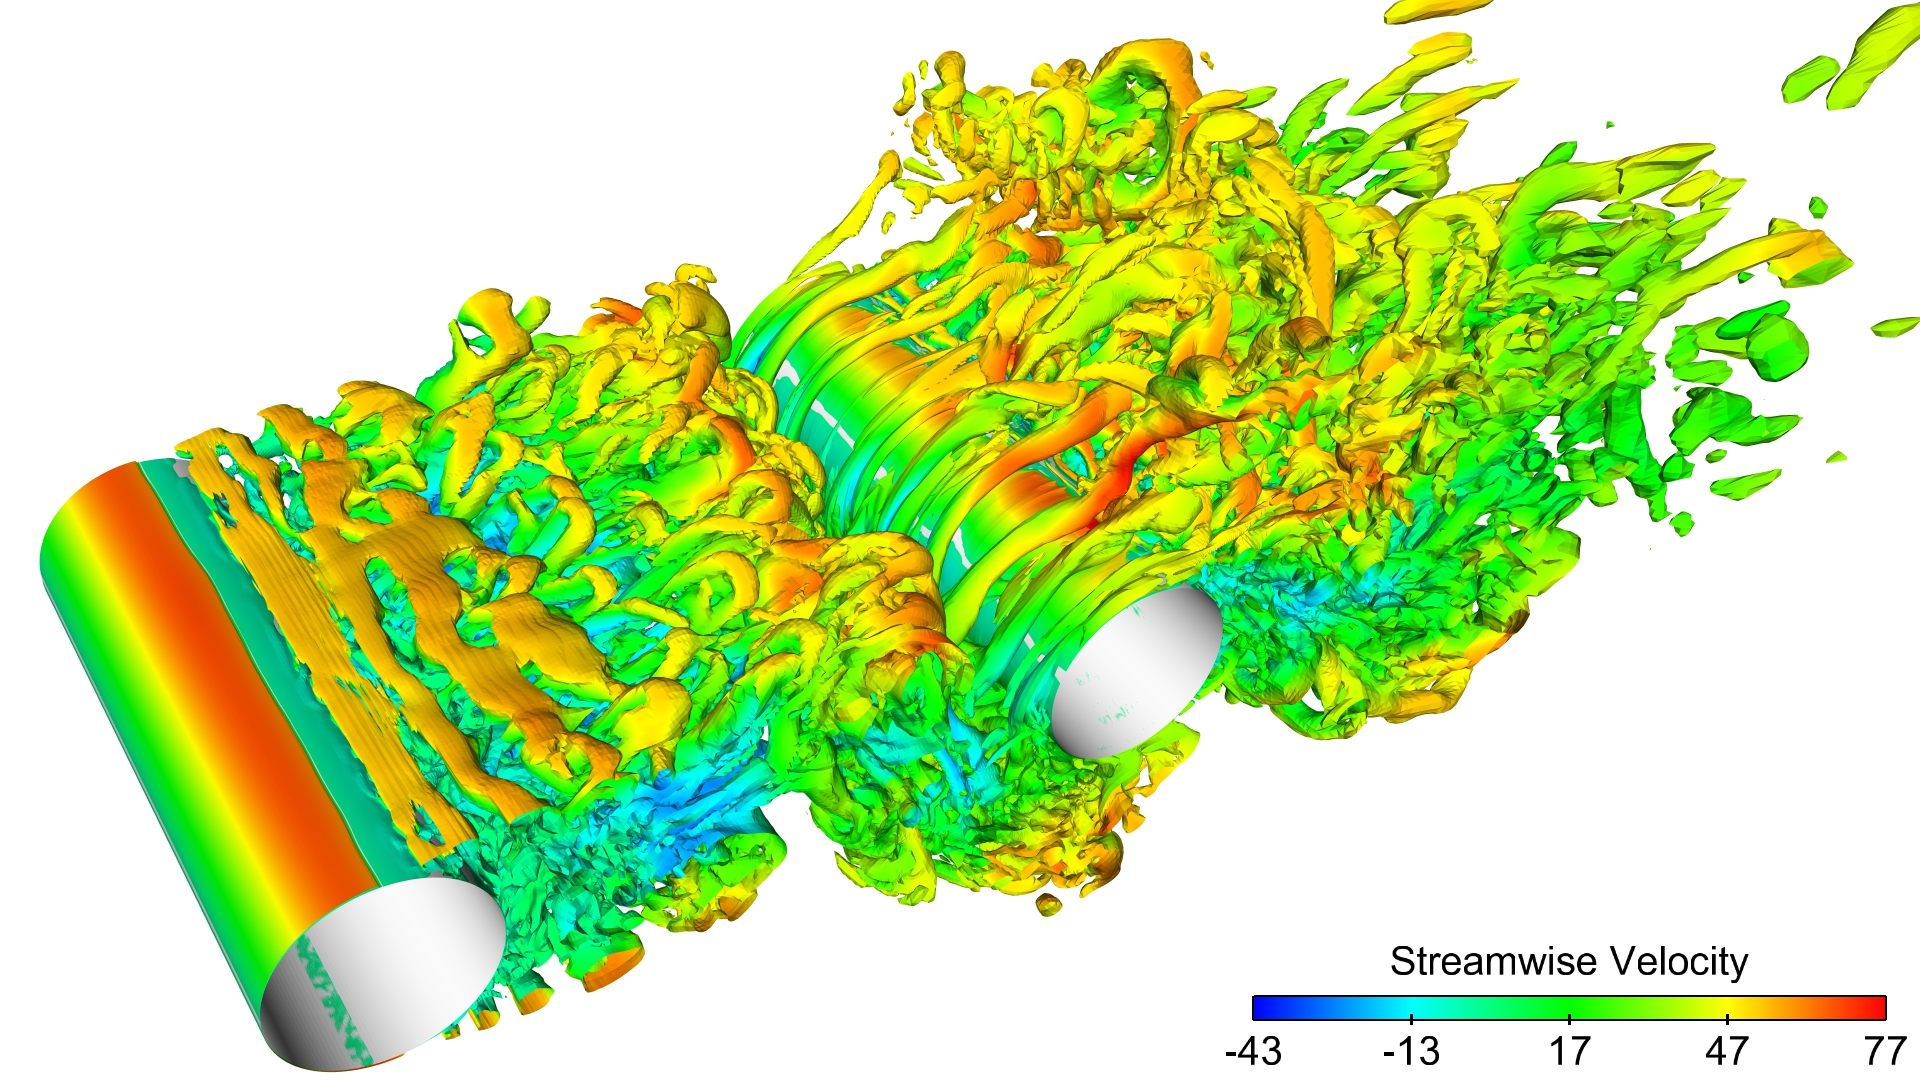
\includegraphics[width=0.45\textwidth]{ITC_Q_Criteria}
            \caption{An Example for including a single figure}
            \label{fig:ITC_Q_Criteria}
        \end{figure}
    \end{verbatim}
\end{center}

\begin{figure}[!htbp]
    \centering
    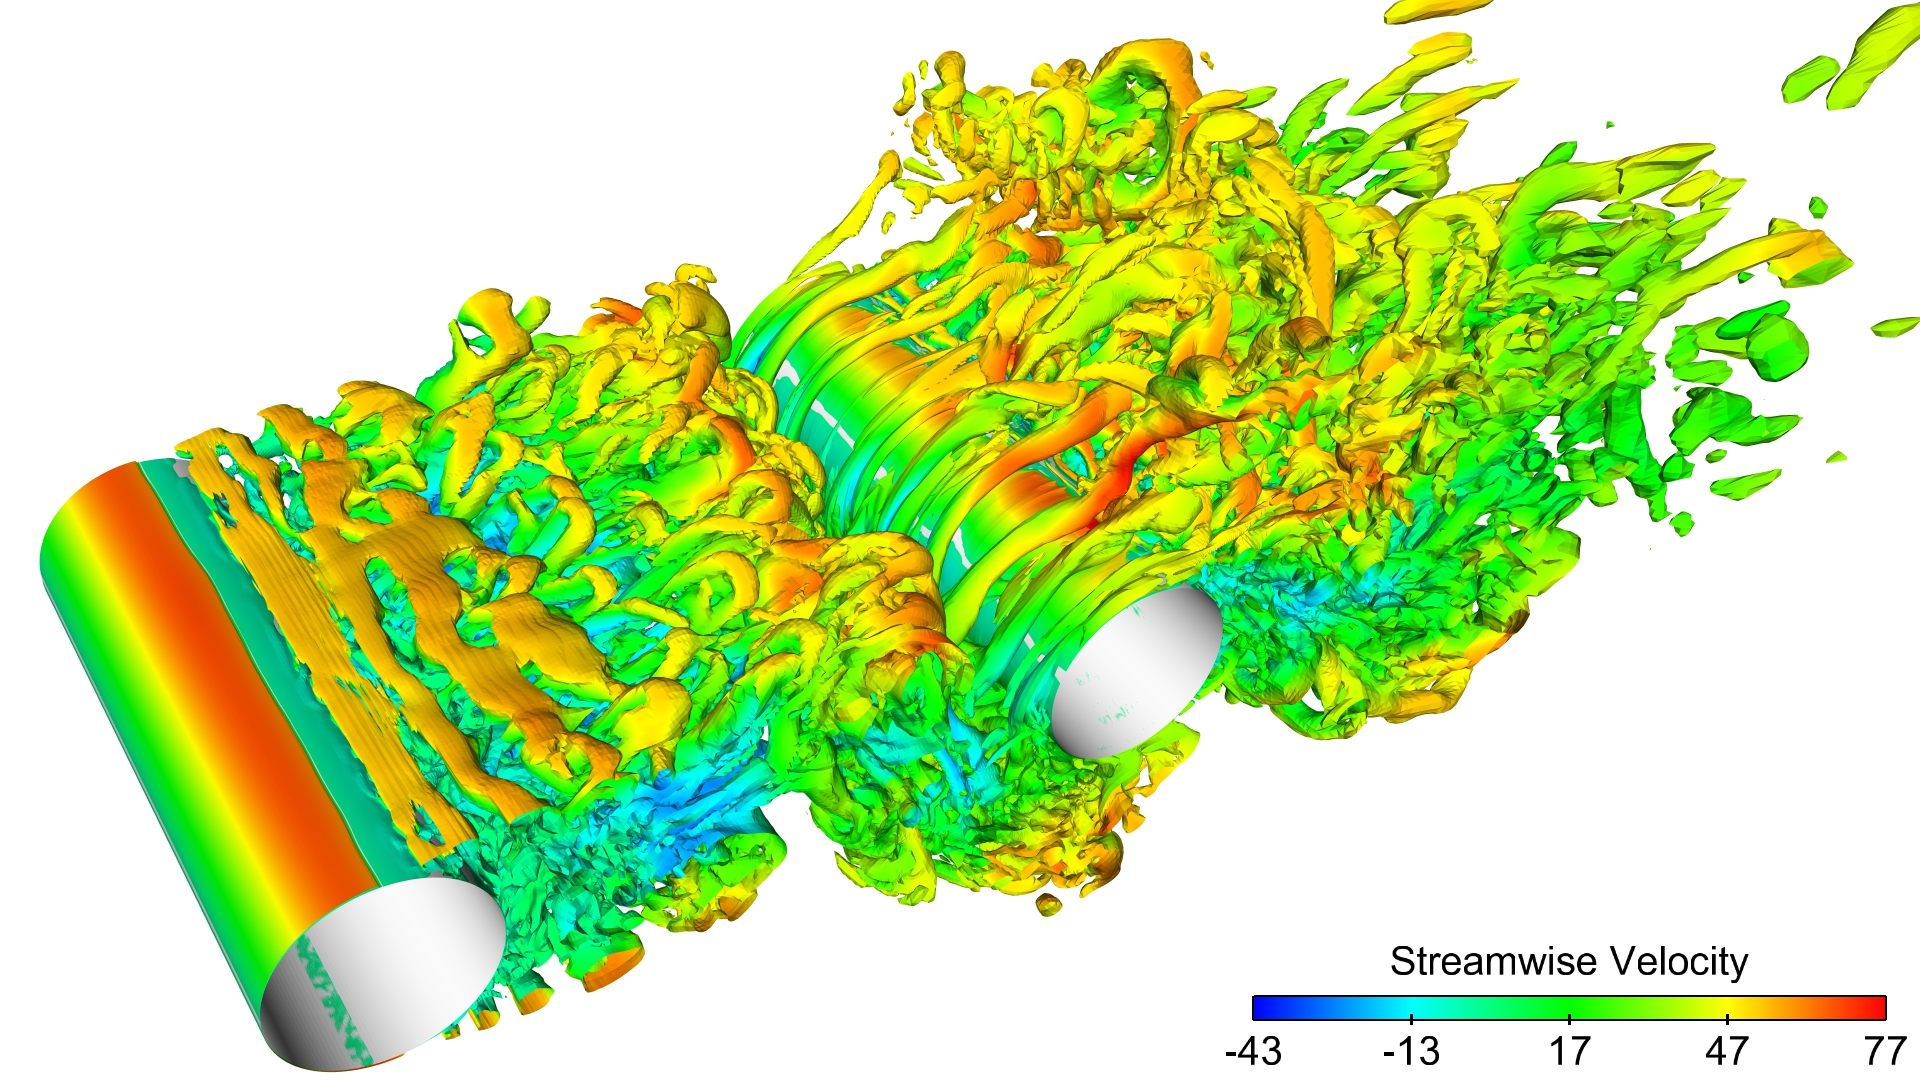
\includegraphics[width=0.45\textwidth]{ITC_Q_Criteria}
    \caption{An Example for including a single graph}
    \label{fig:ITC_Q_Criteria}
\end{figure}

Figure~\ref{fig:HC_OASPL} is an example for including multiple figuress. 
\begin{center}
    \small
    \begin{verbatim}
        \begin{figure}[!htbp]
            \centering
            \begin{subfigure}[b]{0.45\textwidth}
                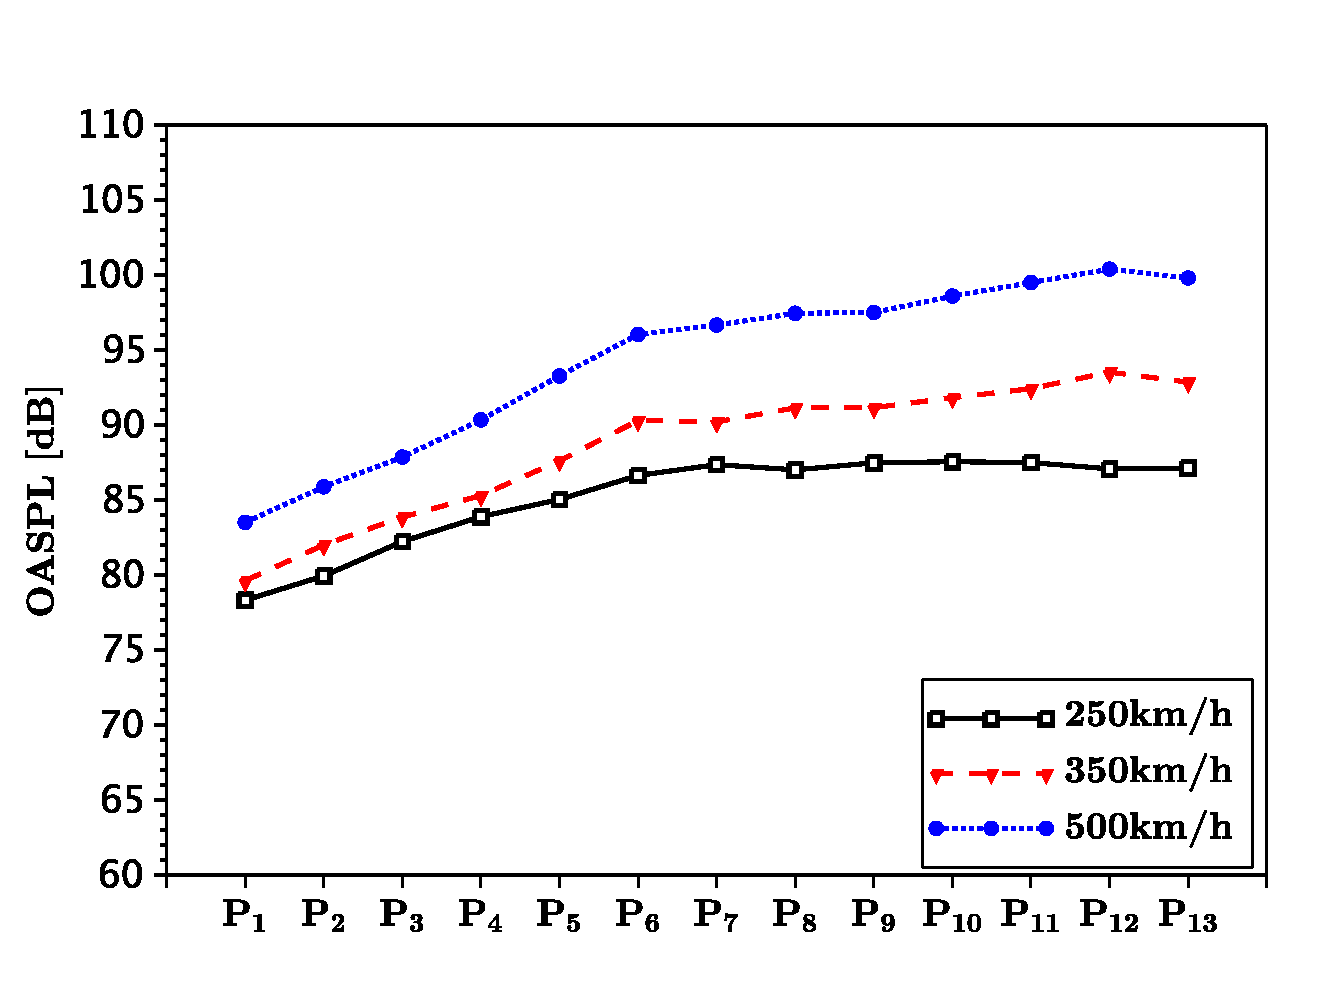
\includegraphics[width=\textwidth]{HC_OASPL_A}
                \caption{}
                \label{fig:HC_OASPL_A}
            \end{subfigure}%
            ~% add a small space
            \begin{subfigure}[b]{0.45\textwidth}
                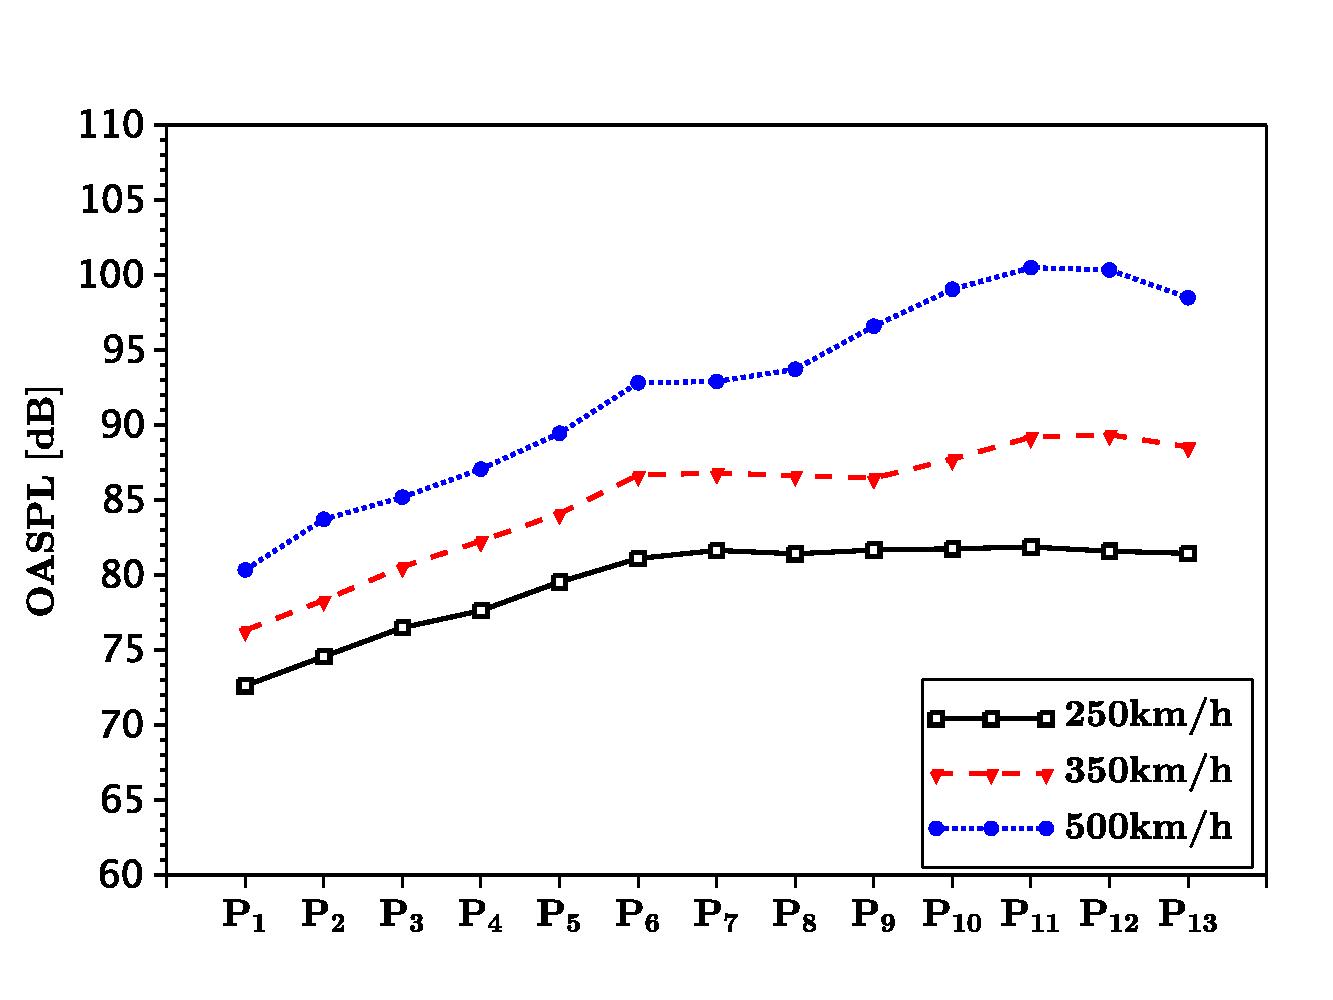
\includegraphics[width=\textwidth]{HC_OASPL_B}
                \caption{}
                \label{fig:HC_OASPL_B}
            \end{subfigure}%
            \\% change line
            \begin{subfigure}[b]{0.45\textwidth}
                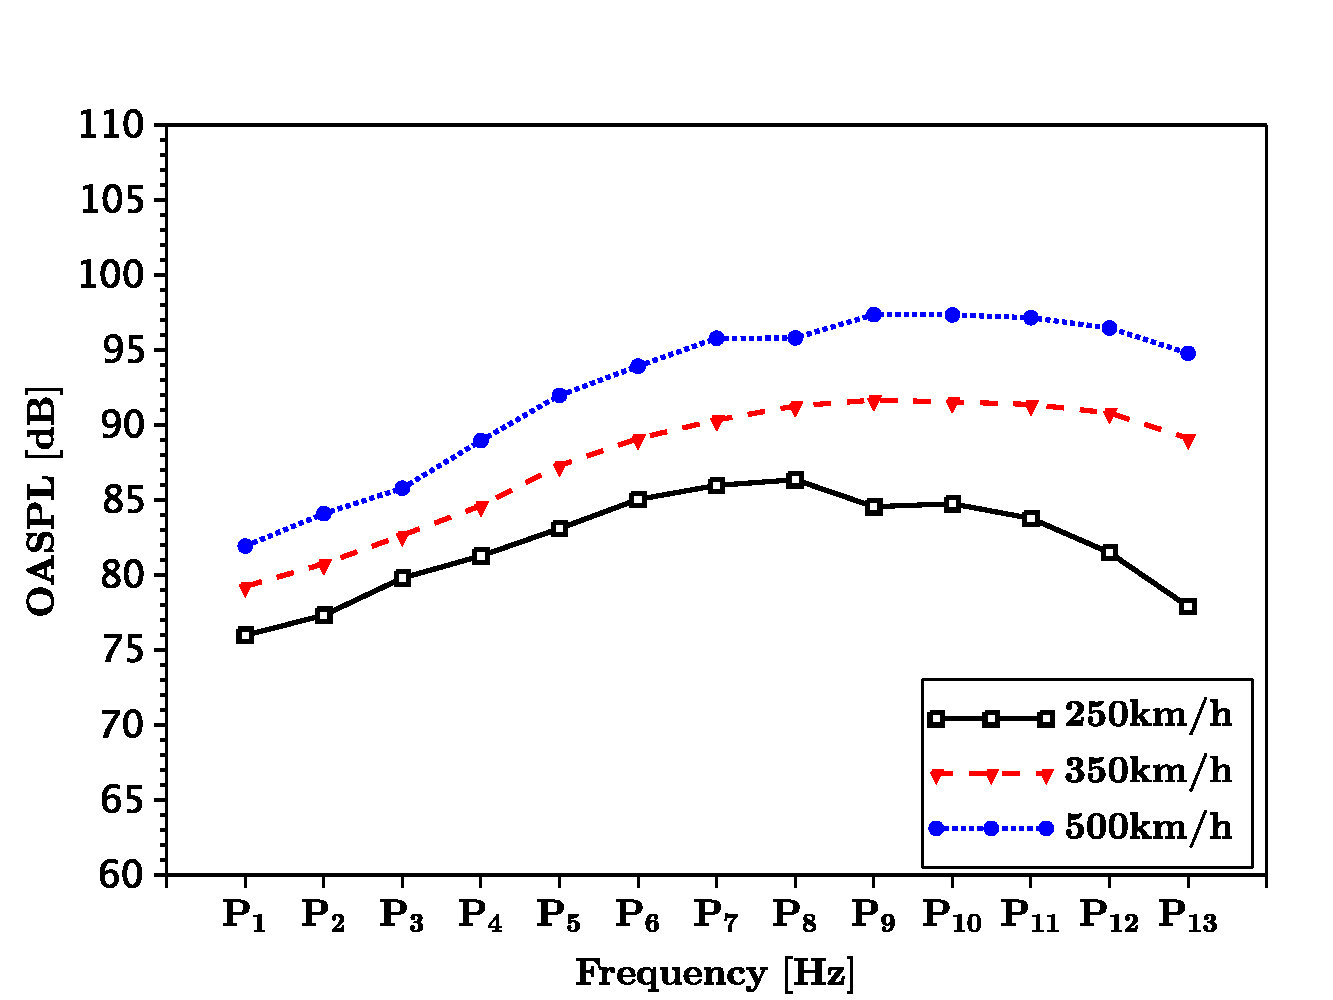
\includegraphics[width=\textwidth]{HC_OASPL_C}
                \caption{}
                \label{fig:HC_OASPL_C}
            \end{subfigure}%
            ~% add a small space
            \begin{subfigure}[b]{0.45\textwidth}
                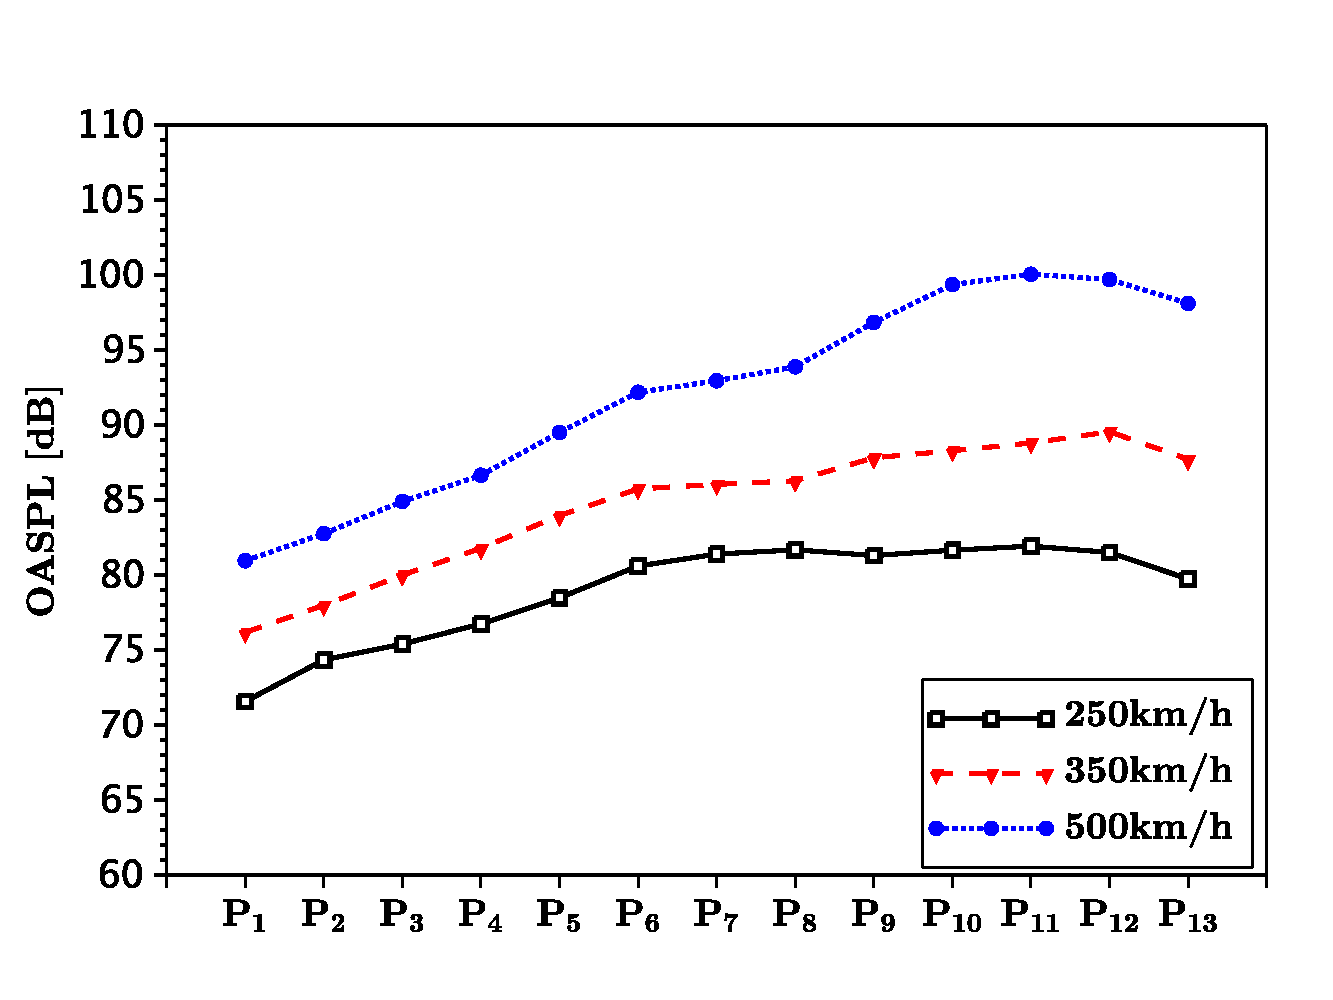
\includegraphics[width=\textwidth]{HC_OASPL_D}
                \caption{}
                \label{fig:HC_OASPL_D}
            \end{subfigure}%
            \caption{An Example for including multiple figures}
            \label{fig:HC_OASPL}
        \end{figure}
    \end{verbatim}
\end{center}
\begin{figure}[!htbp]
    \centering
    \begin{subfigure}[b]{0.45\textwidth}
        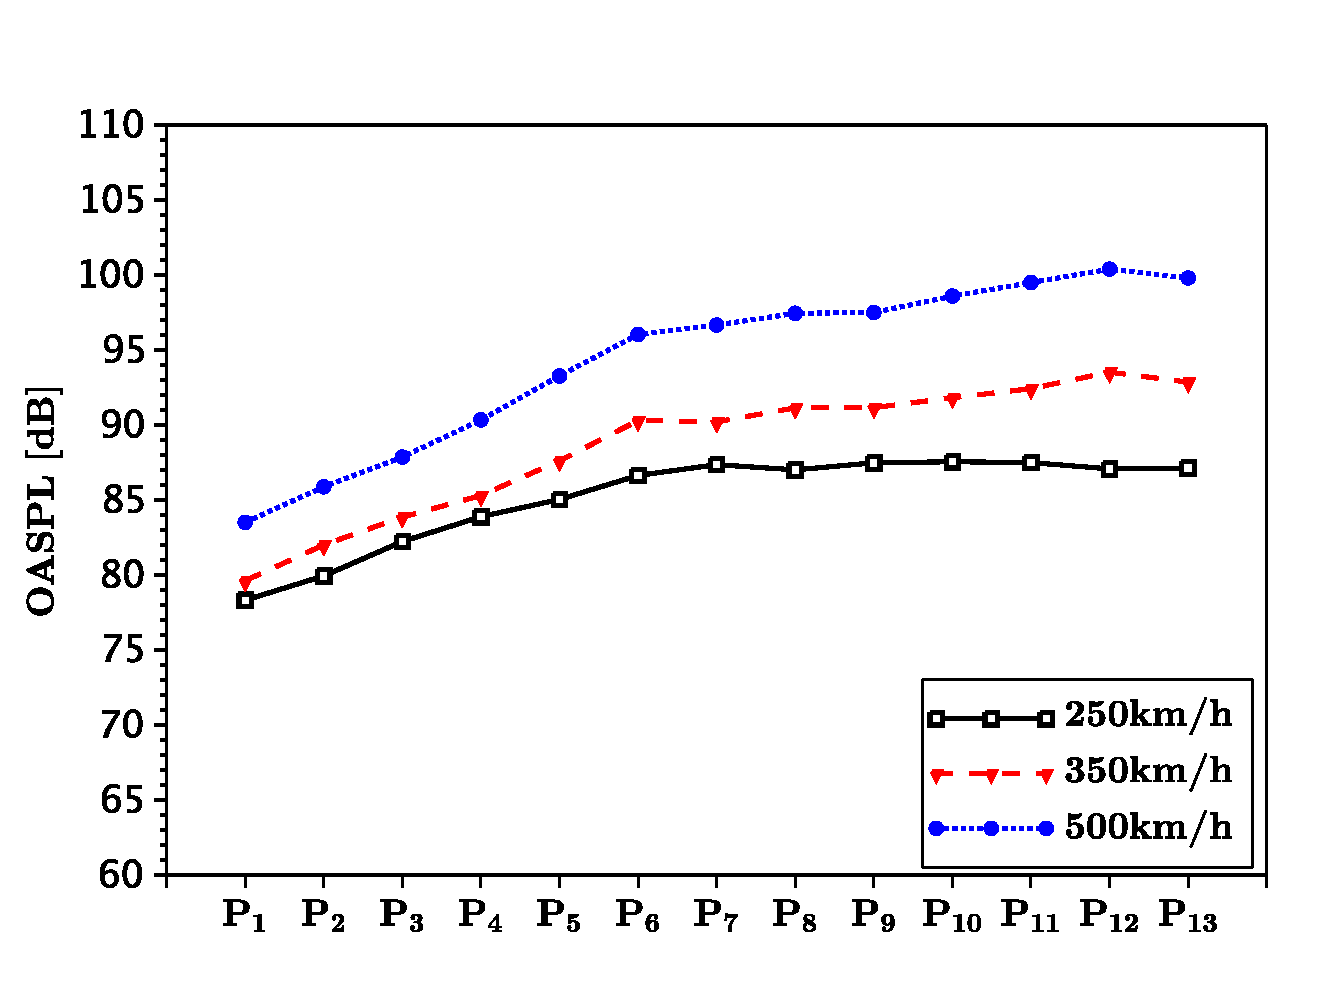
\includegraphics[width=\textwidth]{HC_OASPL_A}
        \caption{}
        \label{fig:HC_OASPL_A}
    \end{subfigure}%
    ~% add a small space
    \begin{subfigure}[b]{0.45\textwidth}
        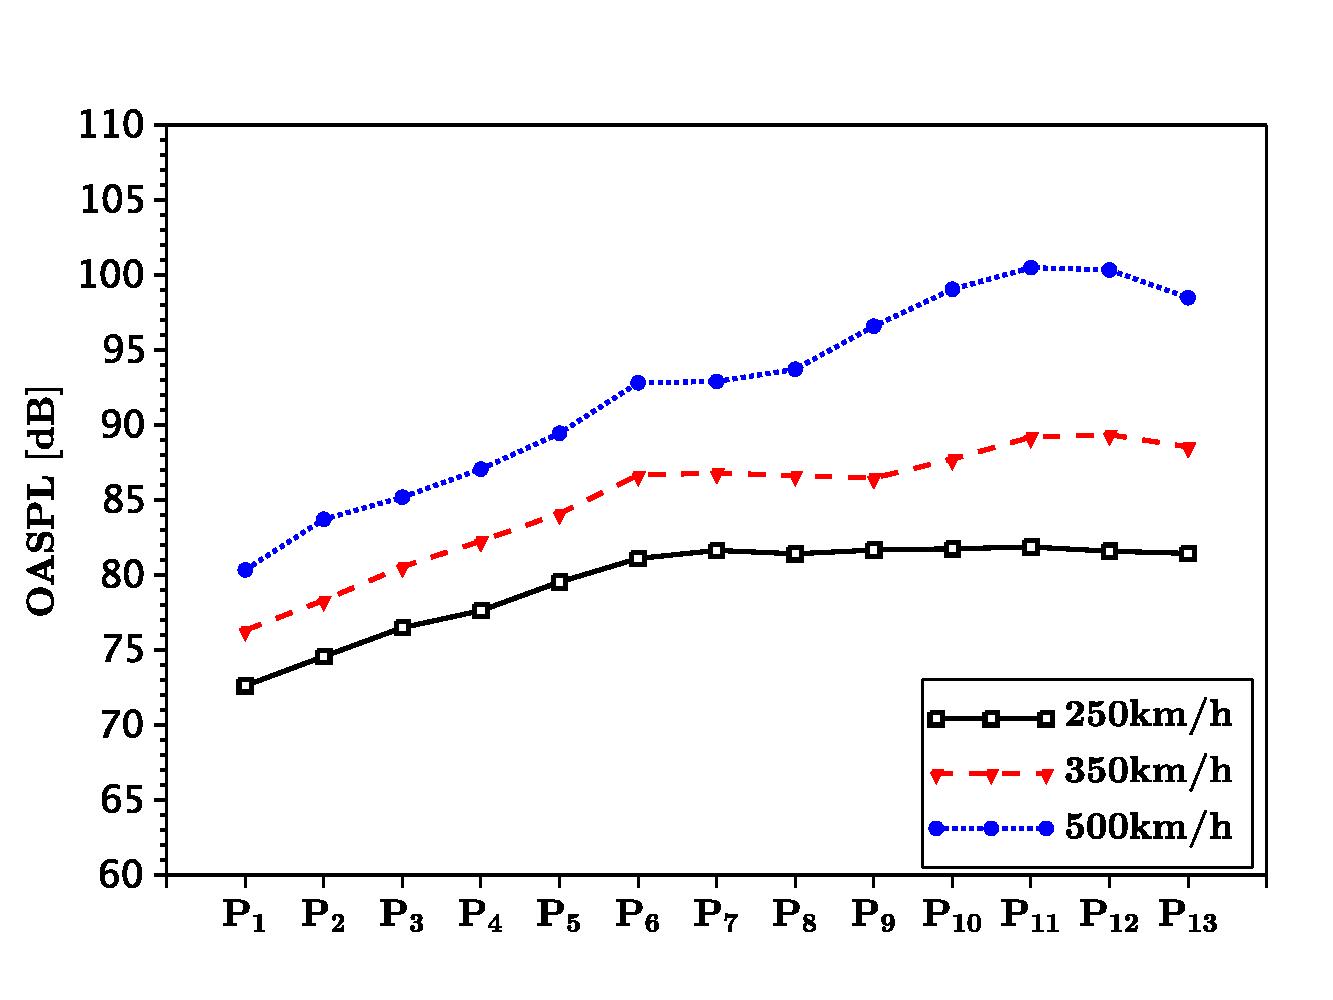
\includegraphics[width=\textwidth]{HC_OASPL_B}
        \caption{}
        \label{fig:HC_OASPL_B}
    \end{subfigure}%
    \\% change line
    \begin{subfigure}[b]{0.45\textwidth}
        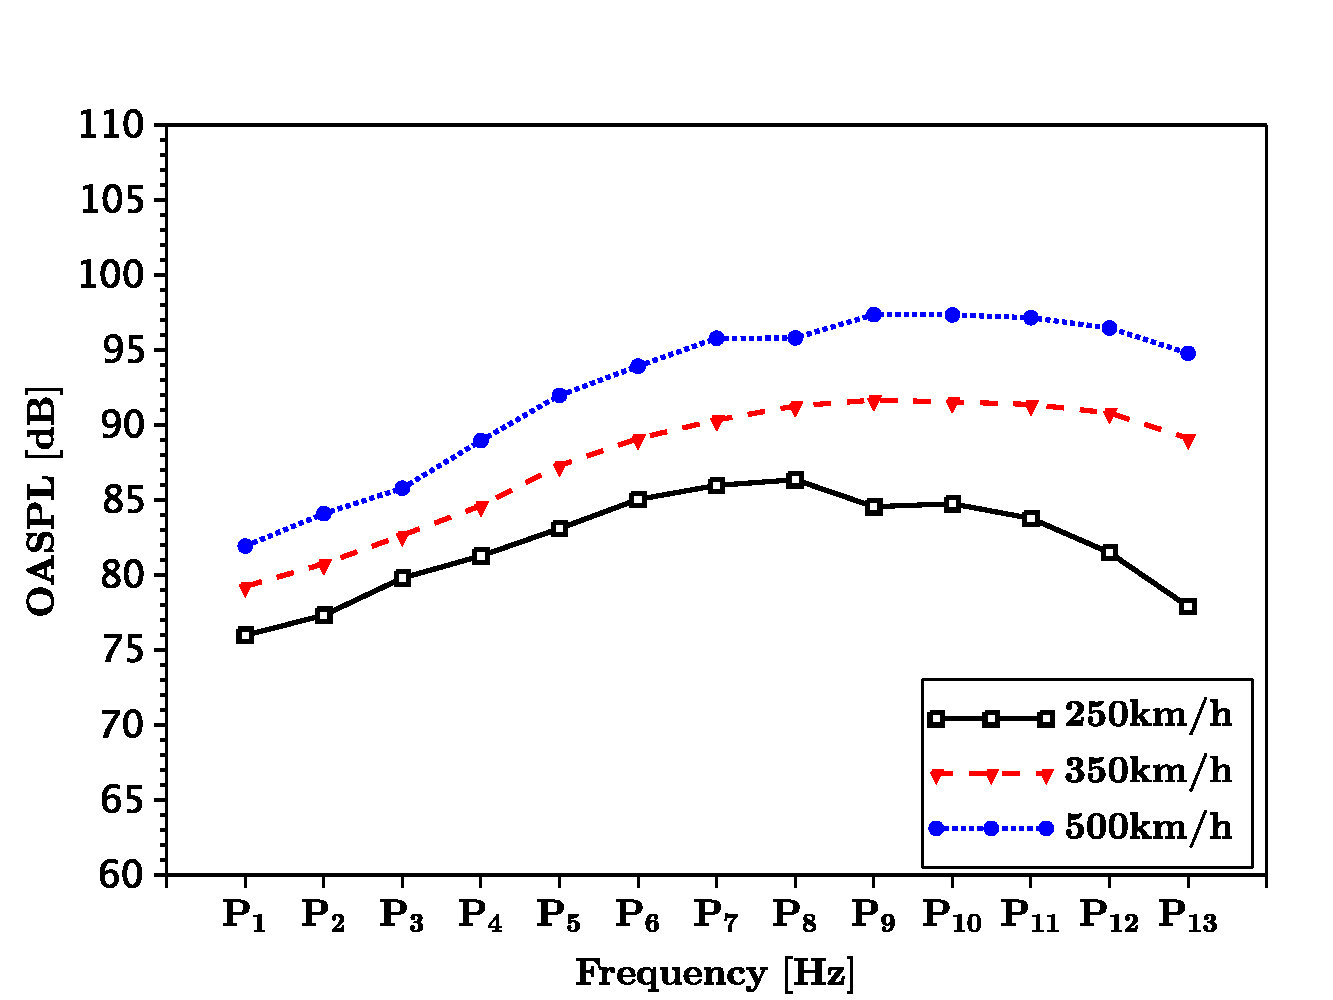
\includegraphics[width=\textwidth]{HC_OASPL_C}
        \caption{}
        \label{fig:HC_OASPL_C}
    \end{subfigure}%
    ~% add a small space
    \begin{subfigure}[b]{0.45\textwidth}
        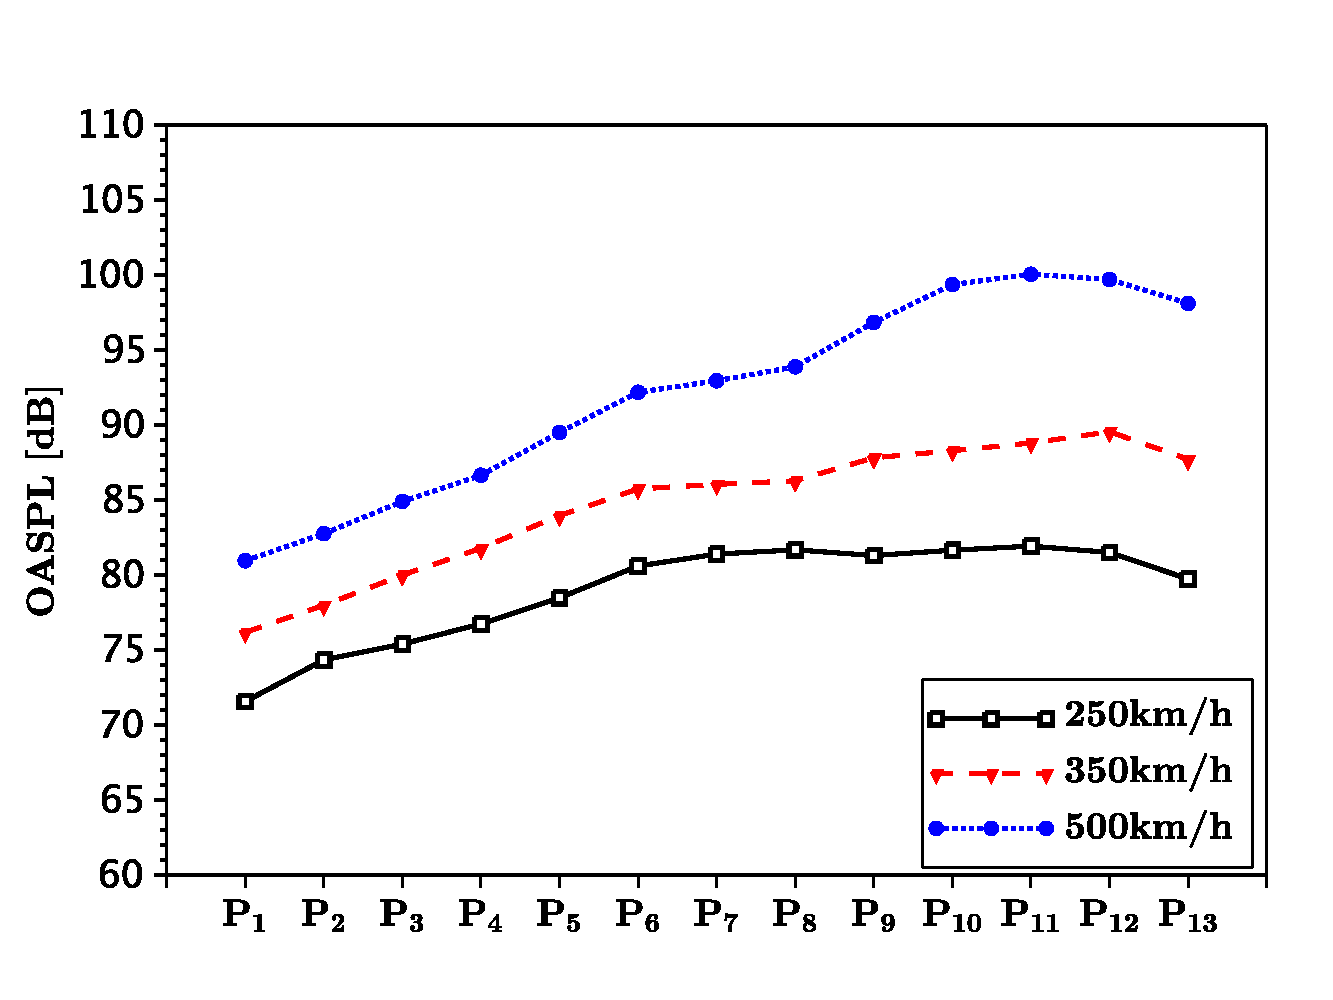
\includegraphics[width=\textwidth]{HC_OASPL_D}
        \caption{}
        \label{fig:HC_OASPL_D}
    \end{subfigure}%
    \caption{An Example for including multiple figures}
    \label{fig:HC_OASPL}
\end{figure}
% subsection Include Graphics (end)

\subsection{Include a citation} % (fold)
Suppose you are going to cite an article named "Document Preparation System", the procedures are:
\begin{itemize}
    \item Use Google Scholar search "Document Preparation System".
    \item Open "Cite" and choose "Import to Bibtex" under the target item.
    \item Copy the citation information of this article into the file "Myrefs.bib"
    \item Research dominant: cite this article by \verb+\citep{lamport1986document}+ like here \citep{lamport1986document}
    \item Citation dominant: cite this article by \verb+\citet{lamport1986document}+ like here \citet{lamport1986document}
    \item References list is generated automatically.
\end{itemize}
% subsection Include a citation (end)
\subsection{Generate nomenclature} % (fold)
In this template, a simple command for adding nomenclatures is provided. Therefore, packages for automatical nomenclature generation are not included. From my point of view, there is no need to use those packages and make things complicated. However, if you insist, there are a lot of available packages for creating nomenclatures. Recommended options are (Please Google the one you want to know):
\begin{itemize}
    \item listofsymbols
    \item nomencl
\end{itemize}
